\documentclass[13pt]{report}
\usepackage[utf8]{vietnam}
\usepackage[T5]{fontenc}
\usepackage{indentfirst}
\usepackage[portrait,left=3.50cm, right=2.50cm, top=2.00cm, bottom=2.00cm]{geometry}
\usepackage[fontsize=13pt]{scrextend}
\usepackage{graphicx}
%\usepackage{amsmath}
\usepackage[linesnumbered,ruled]{algorithm2e}
%\usepackage{algorithm,algorithmic}
\usepackage[ruled]{algorithm2e}
\usepackage{mathrsfs} 
\usepackage{amsfonts}
\usepackage{caption}
\usepackage{subcaption}
\usepackage[pdftex, % Sử dụng PDF TeX
bookmarks=true, % Tạo bookmarks trong tập tin PDF
pdfencoding=auto, % Tự động điều chỉnh encoding của PDF
unicode=true, % Sử dụng Unicode
pdffitwindow=true, % Fit cho vừa cửa sổ
pdfstartview={FitH}, % Zoom file PDF cho vừa khít với nội dung
]{hyperref}

\usepackage{longtable}
\usepackage[intlimits]{amsmath}
\usepackage{amsmath, amsthm, amssymb,latexsym,amscd,amsfonts,enumerate}
\usepackage{fancyhdr}
\usepackage{fancybox,graphicx}
\usepackage[final]{pdfpages}
\usepackage{caption}
\pagestyle{fancy}
\usepackage{tikz}
\usepackage[noend]{algpseudocode}
\usepackage{algpseudocode}
\usepackage[ruled]{algorithm2e}
%\usepackage{subfig}
\usepackage{listings}
%\usepackage[comma,authoryear,round]
%\usepackage{natbib}
\lstset{language=Python}
%\SetAlFnt{\large}
%\SetAlCapFnt{\Large}
%\SetAlCapNameFnt{\Large}
\usepackage[titletoc,toc,page]{appendix}
\usepackage{ upgreek }
\usepackage{bm}
% \newcounter{example}[section]
% \newenvironment{example}[1][]{\refstepcounter{example}\par\medskip
%   \noindent \textbf{Ví dụ~\theexample. #1} \rmfamily}{{\medskip}
%\newtheorem{dn}{Định nghĩa}[section]

%\newtheorem{tc}[dn]{Tính chất}

%\newtheorem{dl}[dn]{Định lí}

%\newtheorem{md}{Mệnh đề}[section]

%\newtheorem{bd}[dn]{Bổ đề}

%\newtheorem{hq}[dn]{Hệ quả}

%\newtheorem{nx}[dn]{Nhận xét}

%\newtheorem{vd}{Ví dụ}[section]

\numberwithin{equation}{section} 


\usetikzlibrary{calc}
\usepackage{titlesec}

\titleformat{\chapter}
{\filcenter\normalfont\Large\bfseries}
{\MakeUppercase{\chaptertitlename}~\thechapter.} {0.5em} {}

%\usepackage{sectsty}
%\chapterfont{\centering}
%\renewcommand\cftpartfont{\LARGE\bfseries}
%\partfont{\Huge}
\fancyhf{}
\rhead{NHÓM 16}
\lhead{BÀI TẬP LỚN CHUỖI THỜI GIAN}
\cfoot{\thepage}
\newtheorem{definition}{Định nghĩa}[chapter]
\renewcommand{\algorithmcfname}{Thuật toán}
\renewcommand{\listalgorithmcfname}{Danh sách thuật toán}
\renewcommand{\baselinestretch}{1.5}


\DeclareMathOperator*{\argmin}{argmin}

\setlength{\parindent}{1cm} % Set khoảng cách thụt đầu dòng mỗi đoạn
\usepackage{epigraph}

\usepackage{tabularx}

\usepackage{ragged2e}
\usepackage{float}
\usepackage{caption}

\usepackage[vietnamese]{babel}
\AtBeginDocument{\renewcommand{\contentsname}{MỤC LỤC}}
\AtBeginDocument{\renewcommand{\listfigurename}{DANH MỤC HÌNH VẼ}}
\AtBeginDocument{\renewcommand{\listtablename}{DANH MỤC BẢNG BIỂU}}
\AtBeginDocument{\renewcommand{\figurename}{{\fontsize{12pt}{0pt}\selectfont \bfseries Hình}}}
\AtBeginDocument{\renewcommand{\thefigure}{{\thechapter.\arabic{figure}}}}
\usepackage[font=bf]{caption}
\captionsetup[figure]{labelsep=space}

\renewcommand{\tablename}{{\fontsize{12pt}{0pt}\selectfont \bfseries Bảng}}
\renewcommand{\thetable}{{\thechapter.\arabic{table}}}
\captionsetup[table]{labelsep=space}

\RequirePackage{listings}
\renewcommand\lstlistlistingname{Danh sách codes}
\definecolor{darkgray}{rgb}{0.66, 0.66, 0.66}
\definecolor{darkorange}{rgb}{1.0, 0.55, 0.0}
\definecolor{gray}{rgb}{0.97,0.97,0.99}
\definecolor{teal}{rgb}{0.0, 0.5, 0.5}
\definecolor{comment}{rgb}{0.6, 0, 0.9}
\lstdefinestyle{mystyle}{
	language = Python,
	backgroundcolor=\color{gray},
	commentstyle=\color{comment},
	keywordstyle=\bfseries\color{darkorange},
	numberstyle=\scriptsize\color{darkgray},
	stringstyle=\color{teal},
	basicstyle=\scriptsize\ttfamily,%\linespread{1}
	breakatwhitespace=false,
	breaklines=true,
	captionpos=t,
	keepspaces=false,
	numbers=left,
	numbersep=3pt,
	showspaces=false,
	showstringspaces=false,
	showtabs=false,
	tabsize=4
}

\lstset{style=mystyle,
literate=%
{À}{{\`A}}1
{Ả}{{\h{A}}}1
{Ã}{{\~A}}1
{Á}{{\'A}}1
{Ạ}{{\d{A}}}1
{Ă}{{\Abreve}}1
{Ằ}{{\`\Abreve}}1
{Ẳ}{{\h\Abreve}}1
{Ẵ}{{\~\Abreve}}1
{Ắ}{{\'\Abreve}}1
{Ặ}{{\d\Abreve}}1
{Â}{{\Acircumflex}}1
{Ầ}{{\'\Acircumflex}}1
{Ẩ}{{\h\Acircumflex}}1
{Ẫ}{{\~\Acircumflex}}1
{Ấ}{{\'\Acircumflex}}1
{Ậ}{{\d\Acircumflex}}1
{Ẩ}{{\h\Acircumflex}}1
{Đ}{{\DJ}}1
{È}{{\`E}}1
{Ẻ}{{\h{E}}}1
{Ẽ}{{\~E}}1
{É}{{\'E}}1
{Ẹ}{{\d{E}}}1
{Ê}{{\Ecircumflex}}1
{Ề}{{\`\Ecircumflex}}1
{Ể}{{\h\Ecircumflex}}1
{Ễ}{{\~\Ecircumflex}}1
{Ế}{{\'\Ecircumflex}}1
{Ệ}{{\d\Ecircumflex}}1
{Ì}{{\`I}}1
{Ỉ}{{\h{I}}}1
{Ĩ}{{\~I}}1
{Í}{{\'I}}1
{Ị}{{\d{I}}}1
{Ò}{{\`O}}1
{Ỏ}{{\h{O}}}1
{Õ}{{\~O}}1
{Ó}{{\'O}}1
{Ọ}{{\d{O}}}1
{Ô}{{\Ocircumflex}}1
{Ồ}{{\`\Ocircumflex}}1
{Ổ}{{\h\Ocircumflex}}1
{Ỗ}{{\~\Ocircumflex}}1
{Ố}{{\'\Ocircumflex}}1
{Ộ}{{\d\Ocircumflex}}1
{Ơ}{{\Ohorn}}1
{Ờ}{{\`\Ohorn}}1
{Ở}{{\h\Ohorn}}1
{Ỡ}{{\~\Ohorn}}1
{Ớ}{{\'\Ohorn}}1
{Ợ}{{\d\Ohorn}}1
{Ù}{{\`U}}1
{Ủ}{{\h{U}}}1
{Ũ}{{\~U}}1
{Ú}{{\'U}}1
{Ụ}{{\d{U}}}1
{Ư}{{\Uhorn}}1
{Ừ}{{\`\Uhorn}}1
{Ử}{{\h\Uhorn}}1
{Ữ}{{\~\Uhorn}}1
{Ứ}{{\'\Uhorn}}1
{Ự}{{\d\Uhorn}}1
{Ỳ}{{\`Y}}1
{Ỷ}{{\h{Y}}}1
{Ỹ}{{\~Y}}1
{Ý}{{\'Y}}1
{Ỵ}{{\d{Y}}}1
{à}{{\`a}}1
{ả}{{\h{a}}}1
{ã}{{\~a}}1
{á}{{\'a}}1
{ạ}{{\d{a}}}1
{ă}{{\abreve}}1
{ằ}{{\`\abreve}}1
{ẳ}{{\h\abreve}}1
{ẵ}{{\~\abreve}}1
{ắ}{{\'\abreve}}1
{ặ}{{\d\abreve}}1
{â}{{\acircumflex}}1
{ầ}{{\`\acircumflex}}1
{ẩ}{{\h\acircumflex}}1
{ẫ}{{\~\acircumflex}}1
{ấ}{{\'\acircumflex}}1
{ậ}{{\d\acircumflex}}1
{ẩ}{{\h\acircumflex}}1
{đ}{{\dj}}1
{è}{{\`e}}1
{ẻ}{{\h{e}}}1
{ẽ}{{\~e}}1
{é}{{\'e}}1
{ẹ}{{\d{e}}}1
{ê}{{\ecircumflex}}1
{ề}{{\`\ecircumflex}}1
{ể}{{\h\ecircumflex}}1
{ễ}{{\~\ecircumflex}}1
{ế}{{\'\ecircumflex}}1
{ệ}{{\d\ecircumflex}}1
{ì}{{\`i}}1
{ỉ}{{\h{i}}}1
{ĩ}{{\~i}}1
{í}{{\'i}}1
{ị}{{\d{i}}}1
{ò}{{\`o}}1
{ỏ}{{\h{o}}}1
{õ}{{\~o}}1
{ó}{{\'o}}1
{ọ}{{\d{o}}}1
{ô}{{\ocircumflex}}1
{ồ}{{\`\ocircumflex}}1
{ổ}{{\h\ocircumflex}}1
{ỗ}{{\~\ocircumflex}}1
{ố}{{\'\ocircumflex}}1
{ộ}{{\d\ocircumflex}}1
{ơ}{{\ohorn}}1
{ờ}{{\`\ohorn}}1
{ở}{{\h\ohorn}}1
{ỡ}{{\~\ohorn}}1
{ớ}{{\'\ohorn}}1
{ợ}{{\d\ohorn}}1
{ù}{{\`u}}1
{ủ}{{\h{u}}}1
{ũ}{{\~u}}1
{ú}{{\'u}}1
{ụ}{{\d{u}}}1
{ư}{{\uhorn}}1
{ừ}{{\`\uhorn}}1
{ử}{{\h\uhorn}}1
{ữ}{{\~\uhorn}}1
{ứ}{{\'\uhorn}}1
{ự}{{\d\uhorn}}1
{ỳ}{{\`y}}1
{ỷ}{{\h{y}}}1
{ỹ}{{\~y}}1
{ý}{{\'y}}1
{ỵ}{{\d{y}}}1
}
\renewcommand{\lstlistingname}{Mã}

\lstset{inputencoding=utf8}


\begin{document}
	\fontsize{13pt}{18pt}\selectfont    %Lệnh thay đổi cỡ chữ thành cỡ 14, cỡ dòng 18 (theo quy chuẩn của Khóa Luận TN).
	
	\setlength{\baselineskip}{18truept}
	\begin{titlepage}                                                       % Đây là trang bìa
		
		%\begin{tikzpicture}[remember picture, overlay]
		% \draw[line width = 4pt] ($(current page.north west) + (1in,-0.7in)$) rectangle ($(current page.south east) + (-0.5in,0.7in)$);
		%\end{tikzpicture}
		\begin{center}
			\fontsize{15pt}{16pt}\selectfont
			{\bf ĐẠI HỌC BÁCH KHOA HÀ NỘI}\\
			%{\bf VIỆN TOÁN ỨNG DỤNG VÀ TIN HỌC}
			%\centerline{--------------------o0o--------------------}  
		\end{center}
		\vspace{3cm}
		\begin{center}
			\fontsize{25pt}{15pt}\selectfont	
			\textbf{BÀI TẬP LỚN \\ CHUỖI THỜI GIAN}\\
		\end{center}
		\vspace{1cm}
		\begin{center}
			\fontsize{23pt}{16pt}\selectfont
			
			\textbf{Mô hình LSTM và mô hình VARMAX trong dự báo chất lượng không khí}  
		\end{center}
		\vspace{0.7cm}
		\begin{center}
			\fontsize{14pt}{16pt}\selectfont 	
			{\bf Phạm Thị Hoa - 20195874}\\	
			\fontsize{14pt}{16pt}\fontsize{14pt}{16pt}\selectfont 	
			{\bf Lê Thanh Thảo - 20195919}\\
			\fontsize{14pt}{16pt}\selectfont 	
			{\bf Phạm Thu Trang - 20195931}\\
			\fontsize{14pt}{16pt}\selectfont
			{\bf Ngành: Toán Tin }\\
			%{\bf Chuyên sâu: Transfer Learning}\\
		\end{center}
		\vspace{2.5 cm}
		\fontsize{13pt}{16pt}\selectfont
		\begin{tabular}
			{@{\hspace{1cm}} l @{\hspace{0.2cm}}p{11.5cm}l}
			
			{\bf Giảng viên hướng dẫn:} &  TS. Nguyễn Thị Ngọc Anh \quad $_{\overline{\text{Chữ kí của GVHD}}}$\\
			{\bf Viện:} &  Toán ứng dụng và Tin học\\
		\end{tabular}
		
		\vspace{3cm}
		\begin{center}
			{\bf HÀ NỘI, 3/2023}
		\end{center}
	\end{titlepage}
	\begin{center}
		\bf Lời cảm ơn\\
	\end{center}
	
	Nhóm chúng em xin gửi lời cảm ơn sâu sắc tới \textbf{TS.Nguyễn Thị Ngọc Anh}, người giảng viên đã tận tình chỉ bảo, luôn theo dõi sát sao và giúp đỡ chúng em trong quá trình nghiên cứu.
    \\

    Chúng em cũng xin gửi lời cảm ơn đến Viện Toán ứng dụng và Tin học, Trường Đại học Bách Khoa Hà Nội đã cung cấp những kiến thức để tạo điều kiện thuận lợi cho chúng em hoàn thành đồ án này.
    \\
    
    Chúng em xin chân thành cảm ơn!
    \thispagestyle{empty}
    \newpage 
	
	\begin{center}
		\bf Tóm tắt nội dung luận văn
	\end{center}
	\par
	Dự báo chuỗi thời gian là một lĩnh vực đã được nghiên cứu từ lâu và được nhiều người quan tâm. Tuy nhiên, trong những năm gần đây, Machine Learning và cụ thể hơn là Deep Learning đang phát triển mạnh mẽ, đạt được nhiều thành tựu vượt trội và thể hiện được nhiều tiềm năng ứng dụng trong chuỗi thời gian. Vì vậy, trong bài tập lớn này, chúng em sẽ tìm hiểu và sử dụng mô hình LSTM và mô hình VARMAX trong bài toán dự đoán chất lượng không khí để có cái nhìn cụ thể hơn về các mô hình này.
    \\
    \textbf{Từ khóa:} \textit{Deep Learning, Long Short-Term Memory (LSTM), Forecasting,Vector Auto Regressive Moving Average with Exogenous variables (VARMAX), Time Series Data.}.%\\
	
	$\qquad\qquad\qquad\qquad\qquad\qquad\qquad\qquad$Hà Nội, ngày 7
	tháng 3 năm 2023
	
	$\qquad\qquad\qquad\qquad\qquad\qquad\quad\qquad\qquad\qquad$Sinh viên thực hiện 
	
	$\qquad\qquad\qquad\qquad\qquad\qquad\qquad\qquad\qquad\hspace{0.5cm} $\textbf{Phạm Thị Hoa}
	
    $\qquad\qquad\qquad\qquad\qquad\qquad\qquad\qquad\qquad\hspace{0.5cm}$\textbf{Lê Thanh Thảo}
    
	$\qquad\qquad\qquad\qquad\qquad\qquad\qquad\qquad\qquad\hspace{0.5cm}$\textbf{Phạm Thu Trang}
	%\chapter*{Tóm tắt nội dung đồ án}
	\thispagestyle{empty}
	\newpage
	\addtocontents{toc}{{\protect\thispagestyle{empty}}}
	\tableofcontents
	\thispagestyle{empty}
	\newpage
	%\listoffigures
	
	{\let\oldnumberline\numberline
\renewcommand{\numberline}{Hình~\oldnumberline}
\listoffigures} 
\thispagestyle{empty}
\newpage
	
	\newpage
	%\listoftables
	{\let\oldnumberline\numberline
\renewcommand{\numberline}{Bảng~\oldnumberline}
\listoftables}
\thispagestyle{empty}
	\newpage
	\newpage
	\chapter*{DANH MỤC KÍ HIỆU VÀ CHỮ VIẾT TẮT}
	\begin{table}[htp]
		\centering
		\begin{tabular}{ll}
			
			\textbf{Từ viết tắt} & \textbf{Ý nghĩa}\\
			LSTM & Long short-term memory \\
                VARMAX & Vector Auto Regressive Moving Average \\ 
                 & with Exogenous variables\\
    		RNN & Recurrent Neural Network\\
    		ML & Machine Learning\\
    		DL & Deep Learning\\
		\end{tabular}
	\end{table}~
\\
\thispagestyle{empty}
	\newpage
	\pagenumbering{arabic}
\setcounter{page}{1}
\chapter{MỞ ĐẦU}
\section{Lời mở đầu}
Con người có thể sống sót trong 30 ngày mà không cần ăn, 3 ngày không uống, nhưng sẽ chết chỉ sau 3 phút nếu không thở. Nhu cầu về không khí của con người cũng không đổi, chúng ta hít thở nó thường xuyên dù trong nhà hay ngoài nhà, thậm chí phải chấp nhận cả khi chất lượng không được như mong đợi. Mùi khó chịu khiến con người nhận ra chất lượng không khí không tốt, nhưng nhiều khi khứu giác lại không thể cảm nhận được những tác nhân gây hại đang tồn tại, như các hóa chất độc hại – chúng ảnh hưởng vô cùng tồi tệ tới sức khỏe.

Ngày này chất lượng không khí tại các thành phố lớn ngày càng đi xuống. Bởi vậy việc đo lường, dự đoán chất lượng không khí tại một khu vực nhất định là vô cùng cần thiết. Nó cho ta biết chỉ số ô nhiễm tại nơi đó là bao nhiêu, nếu chỉ số quá cao sẽ ảnh hưởng rất lớn tới sức khỏe con người. 

\section{Giới thiệu bài toán}
\begin{itemize}
    \item [$-$]Bài toán: Nhóm chúng em sẽ sử dụng mô hình LSTM và mô hình VARMAX để dự đoán chất lượng không khí trong 24h tới dựa vào các thông số thời tiết của các ngày trước đó như: nhiệt độ, độ ẩm, hướng gió, áp suất khí quyển, lượng bụi mịn PM10, PM 2.5, nồng độ khí CO, S02, NO trong không khí,...

    \item [$-$]Phạm vi nghiên cứu: từ ngày 14/4/2015 tới ngày 5/9/2019.
\end{itemize}

\newpage
\section{Phân công công việc trong nhóm}
\begin{table}[h!]
    \centering
    \tabcolsep = 0.1cm
    \begin{tabular}{|c|c|}
        \hline
        \textbf{Sinh viên} & \textbf{Công việc}\\ 
        \hline
        Phạm Thị Hoa & Tìm hiểu code và ứng dụng mô hình LSTM vào bài toán\\
        \hline
        Lê Thanh Thảo & Tìm hiểu các mô hình và làm báo cáo\\
        \hline
        Phạm Thu Trang & Tìm hiểu code và ứng dụng mô hình VARMAX vào bài toán\\ 
        \hline
    \end{tabular}
    \caption{Phân công công việc}
    %\label{tab:my_label}
\end{table}
	\chapter{CƠ SỞ LÝ THUYẾT}
\subsection{Mạng nơ-ron đệ quy (RNN)}
\subsubsection{Kiến trúc mạng nơ-ron đệ quy RNN}
Con người không bắt đầu suy nghĩ của họ từ đầu tại tất cả các thời điểm. Cũng giống như việc đọc báo cáo đồ án này, chúng ta hiểu mỗi chữ ở đây dựa vào các chữ chúng ta đã hiểu trước đó chứ không phải đọc tới đâu ném hết đi tới đó, rồi bắt đầu suy nghĩ lại từ đầu tới chữ chúng ta đang đọc. Tức là tư duy đã có bộ nhớ để lưu lại những gì điễn ra trước đó.\par
Tuy nhiên các mô hình mạng nơ-ron truyền thống thì không thể làm được việc đó, đó có thể coi là một khuyết điểm chính của mạng nơ-ron truyền thống. Ví dụ, nếu chúng ta muốn phân loại các bối cảnh xảy ra ở tất cả các thời điểm trong một bộ phim, thì đúng là không thể hiểu được một tình huống trong phim mà lại phụ thuộc vào các tình huống trước đó nếu sử dụng các mạng nơ-ron truyền thống.\par
Mạng nơ-ron hồi quy (Recurrent Neural Network) sinh ra để giải quyết vấn đề đó. Mạng này chứa các vòng lặp bên trong cho phép thông tin có thể lưu lại được.\par
\begin{figure}[H]
    \centering
    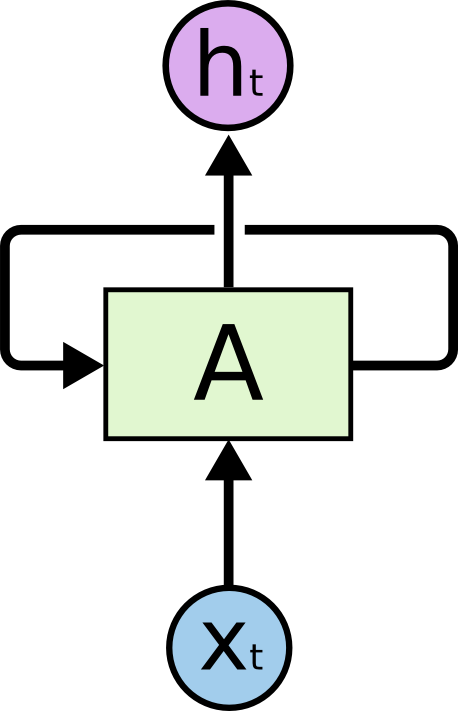
\includegraphics[scale=0.5]{figures/RNN-rolled.png}
    \caption{Recurrent Neural Networks have loops.}
\end{figure}
Hình vẽ trên mô tả một đoạn của mạng nơ-ron hồi quy $\mathcal{A}$ với đầu vào là $x_t$ và đầu ra là $h_t$. Một vòng lặp cho phép thông tin có thể được truyền từ bước này qua bước này qua bước khác của mạng nơ-ron.\par
Một mạng nơ-ron hồi quy có thể được coi là nhiều bản sao chép của cùng một mạng, trong đó mỗi đầu ra của mạng này là đầu vào của một mạng sao chép khác. Chuỗi lặp lại các mạng này chính là phân giải của mạng nơ-ron hồi quy, các vòng lặp khiến chúng tạo thành một chuỗi danh sách các mạng sao chép nhau. \par
\begin{figure}[H]
    \centering
    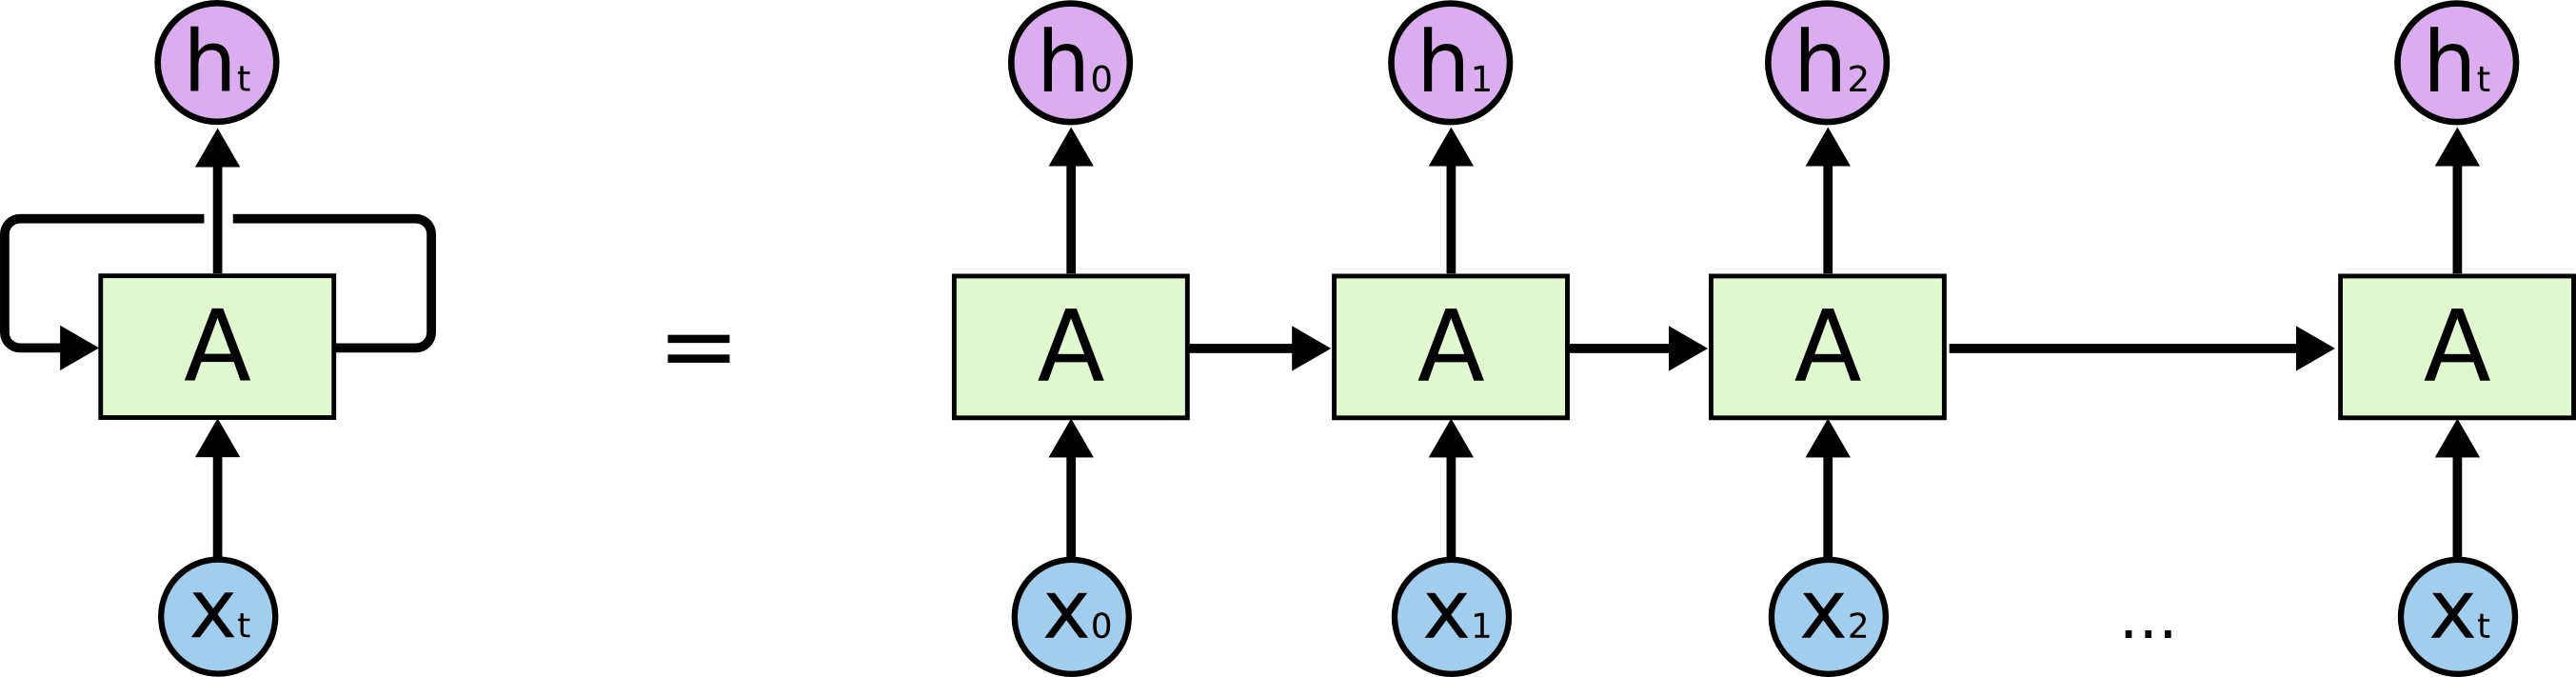
\includegraphics[width=0.75\textwidth]{figures/RNN-unrolled.png}
    \caption{An unrolled recurrent neural network.}
\end{figure}
Trong vài năm gần đây, việc ứng dụng RNN đã đưa ra được nhiều kết quả không thể tin nổi trong nhiều lĩnh vực: nhận dạng giọng nói, mô hình hóa ngôn ngữ, dịch máy, mô tả ảnh,… Danh sách vẫn còn đang được mở rộng tiếp.
\subsubsection{Vấn đề phụ thuộc xa}
Một điểm nổi bật của RNN chính là ý tưởng kết nối các thông tin phía trước để dự đoán cho hiện tại. Việc này tương tự như ta sử dụng các cảnh trước của bộ phim để hiểu được cảnh hiện thời. Nếu mà RNN có thể làm được việc đó thì chúng sẽ cực kì hữu dụng, tuy nhiên liệu chúng có thể làm được không?\par
Đôi lúc ta chỉ cần xem lại thông tin vừa có thôi là đủ để biết được tình huống hiện tại. Ví dụ, ta có câu: \textit{“các đám mây trên bầu trời”} thì ta chỉ cần đọc tới \textit{“các đám mây trên bầu”} là đủ biết được chữ tiếp theo là \textit{“trời”} rồi. Trong tình huống này, khoảng cách tới thông tin có được cần để dự đoán là nhỏ, nên RNN hoàn toàn có thể học được.\par
\begin{figure}[H]
    \centering
    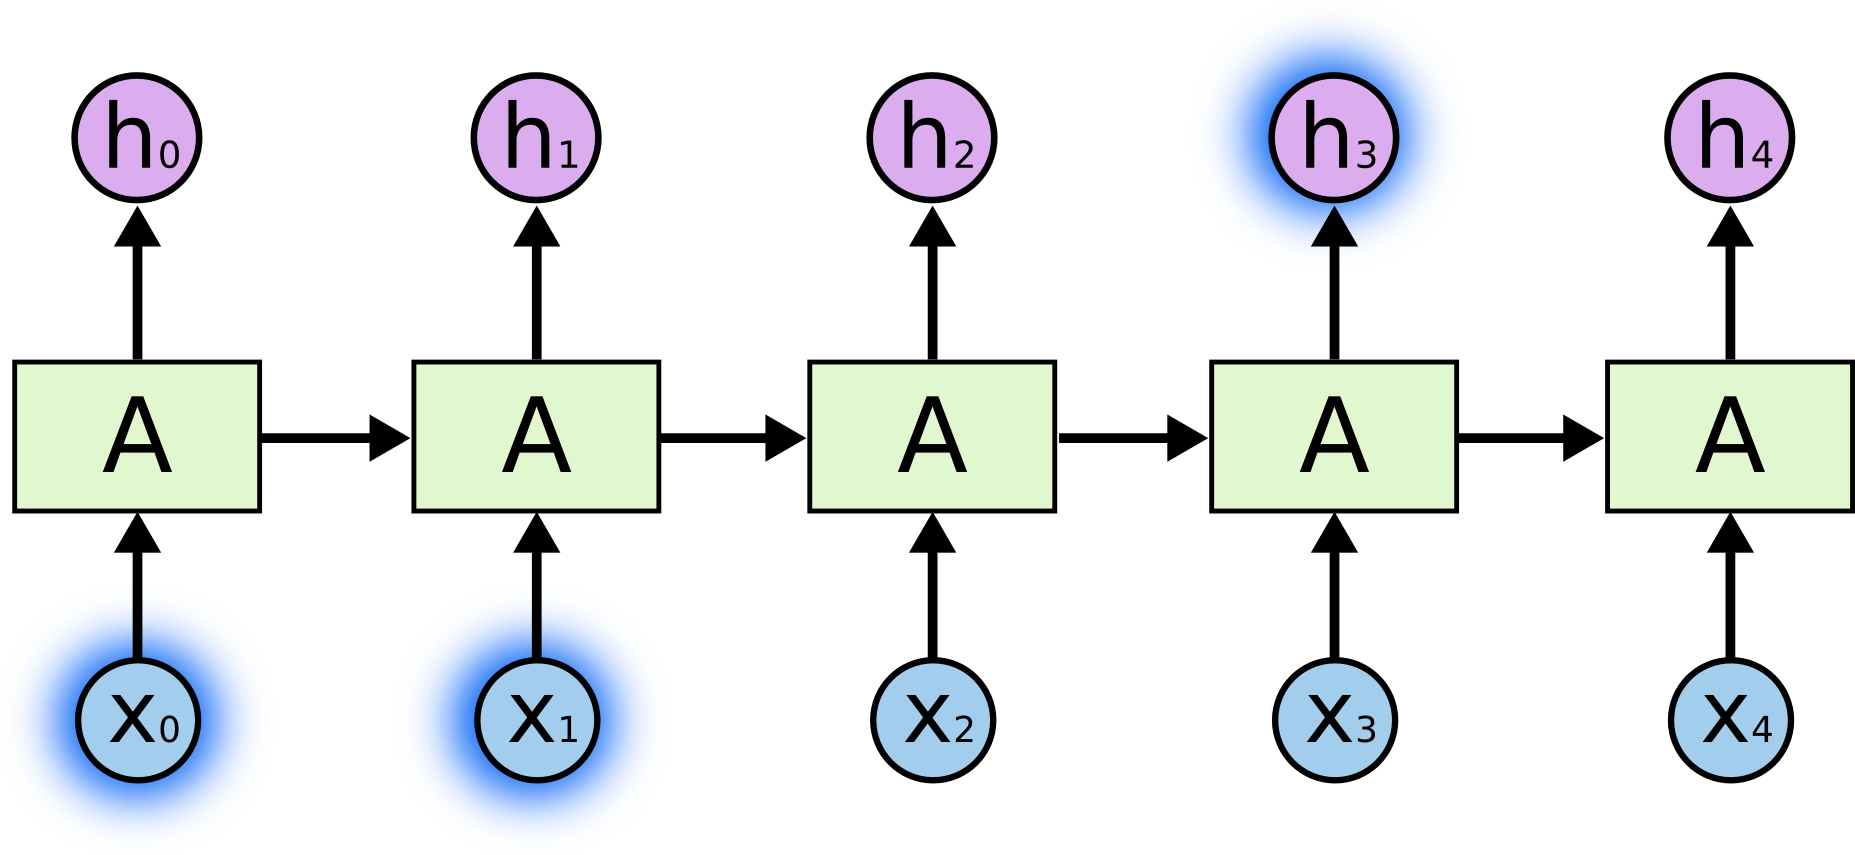
\includegraphics[width=0.7\textwidth]{figures/RNN-shorttermdepdencies.png}
    \caption{Mạng RNN phụ thuộc ngắn.}
\end{figure}
Nhưng trong nhiều tình huống ta buộc phải sử dụng nhiều ngữ cảnh hơn để suy luận. Ví dụ, dự đoán chữ cuối cùng trong đoạn: \textit{“I grew up in France… I speak fluent French.”}. Rõ ràng là các thông tin gần (\textit{”I speak fluent”}) chỉ có phép ta biết được đằng sau nó sẽ là tên của một ngôn ngữ nào đó, còn không thể nào biết được đó là tiếng gì. Muốn biết là tiếng gì, thì ta cần phải có thêm ngữ cảnh \textit{“I grew up in France”} nữa mới có thể suy luận được. Rõ ràng là khoảng cách thông tin lúc này có thể đã khá xa rồi.\par
Thật không may là với khoảng cách càng lớn dần thì RNN bắt đầu không thể nhớ và học được nữa.
\begin{figure}[H]
    \centering
    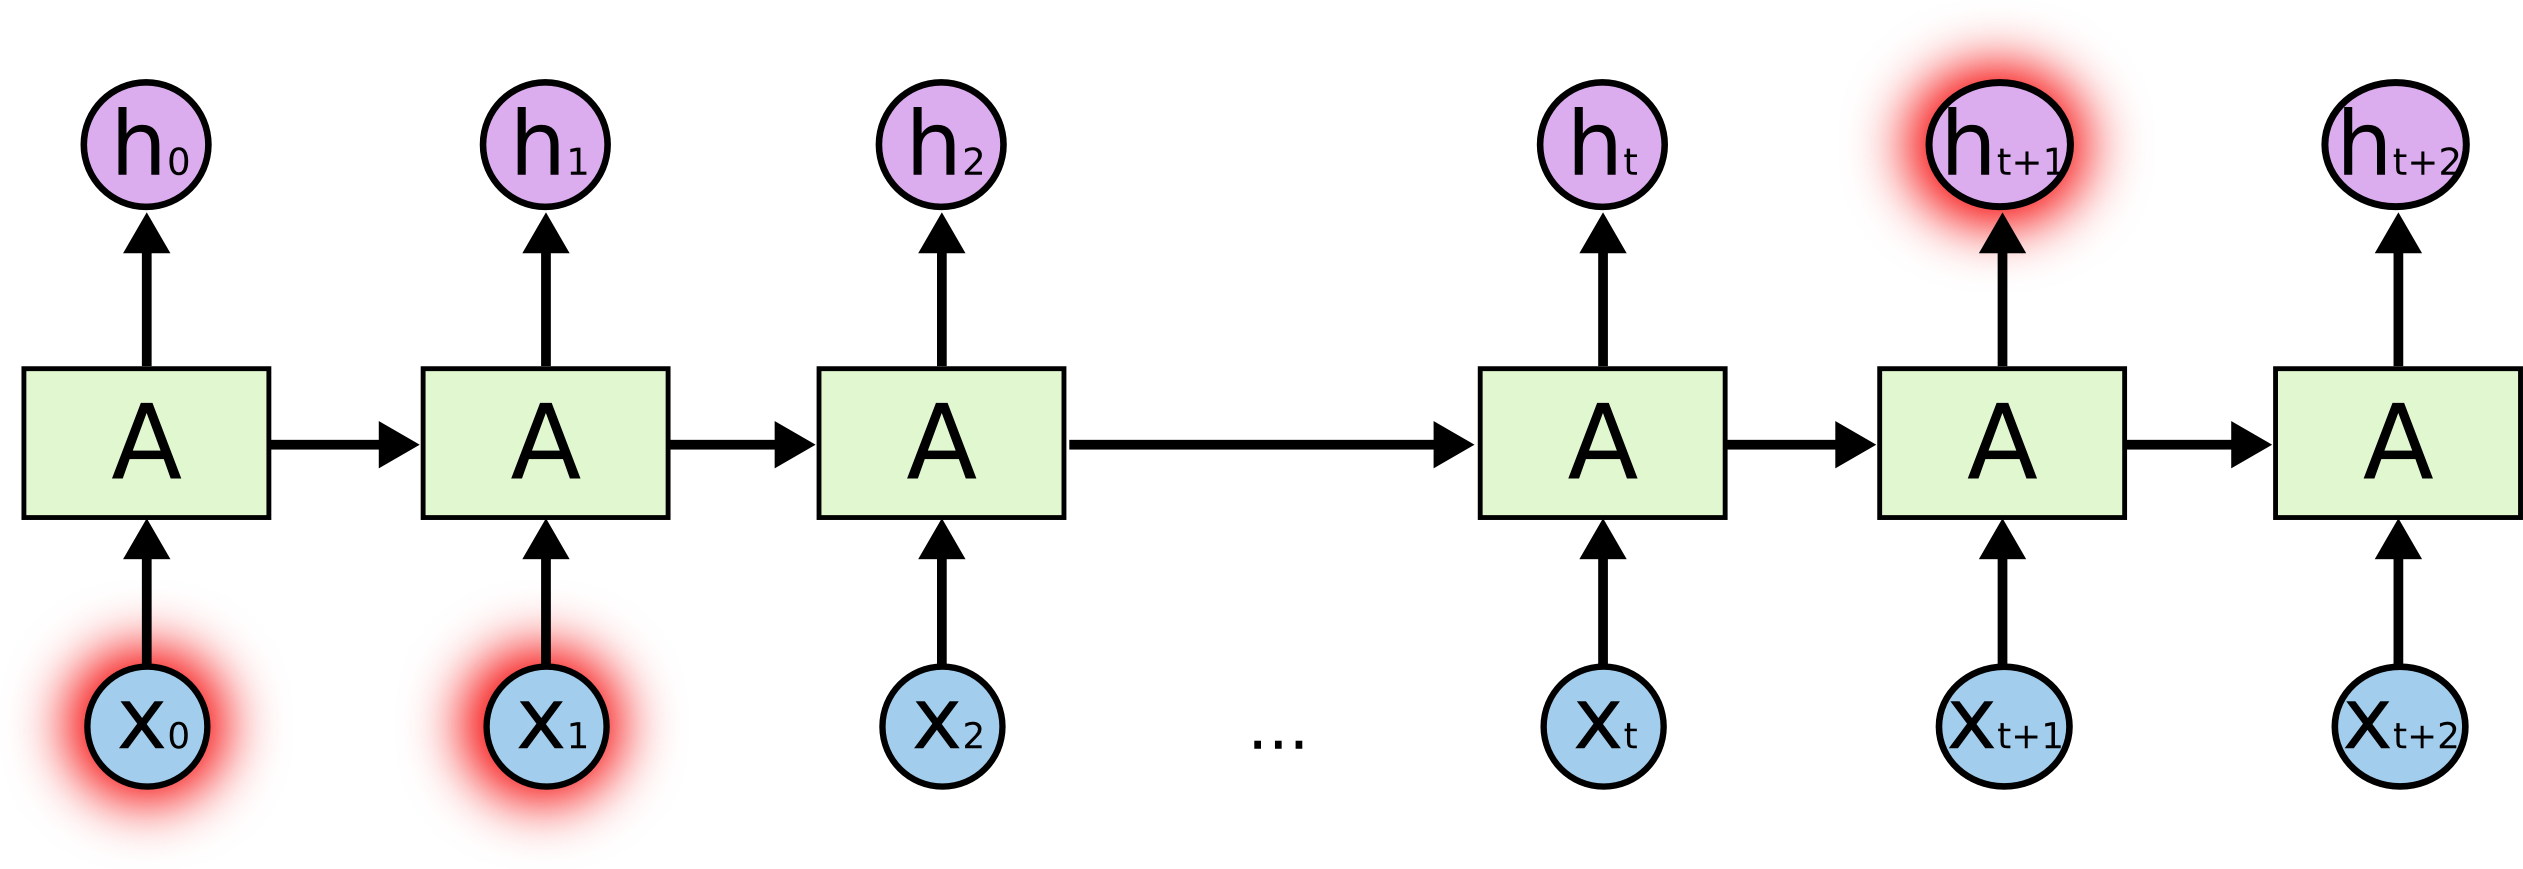
\includegraphics[width=0.75\textwidth]{figures/RNN-longtermdependencies.png}
    \caption{Mạng RNN phụ thuộc dài.}
\end{figure}
Về mặt lý thuyết, rõ ràng là RNN có khả năng xử lý các phụ thuộc xa (long-term dependencies). Chúng ta có thể xem xét và cài đặt các tham số sao cho khéo là có thể giải quyết được vấn đề này. Tuy nhiên, đáng tiếc trong thực tế RNN có vẻ không thể học được các tham số đó. Vấn đề này đã được khám phá khá sâu bởi \textbf{Hochreiter (1991)} và \textbf{Bengio, et al (1994)} trong các bài báo của mình, họ đã tìm được nhưng lý do căn bản để giải thích tại sao RNN không thể học được. \par
Tuy nhiên, LSTM không vấp phải vấn đề đó.
\section{LSTM}
\subsection{Mô hình Long Short Term Memory networks (LSTM)}
Mạng bộ nhớ dài-ngắn (Long Short Term Memory networks), thường được gọi là LSTM - là một phiên bản mở rộng của mạng thần kinh hồi quy (RNN) nhân tạo được sử dụng trong lĩnh vực học sâu. LSTM được giới thiệu bởi \textbf{Hochreiter \& Schmidhuber}  vào năm 1997.\par
LSTM được đưa ra để giải quyết các vấn đề về phụ thuộc xa (long-term dependency) trong mạng RNN do bị ảnh hưởng bởi vấn đề mất gradient. Việc nhớ thông tin trong suốt thời gian dài là đặc tính mặc định của LSTM, chứ không cần phải huấn luyện để có thể nhớ được. Tức là ngay nội tại của nó đã có thể ghi nhớ được mà không cần bất kì can thiệp nào.\par

Một đơn vị LSTM thông thường bao gồm:
\begin{itemize}
    \item \textbf{Tế bào (cell)}
    \item \textbf{Cổng quên (forget gate):} có nhiệm vụ loại bỏ những thông tin không cần thiết nhận được khỏi cell internal state.
    \item \textbf{Cổng vào (input gate):} có nhiệm vụ chọn lọc nhưng thông tin cần thiết nào được thêm vào cell internal state.
    \item \textbf{Cổng ra (output gate):} có nhiệm vụ xác định những thông tin nào từ cell internal state được sử dụng như đầu ra.
\end{itemize}
\begin{figure}[H]
    \centering
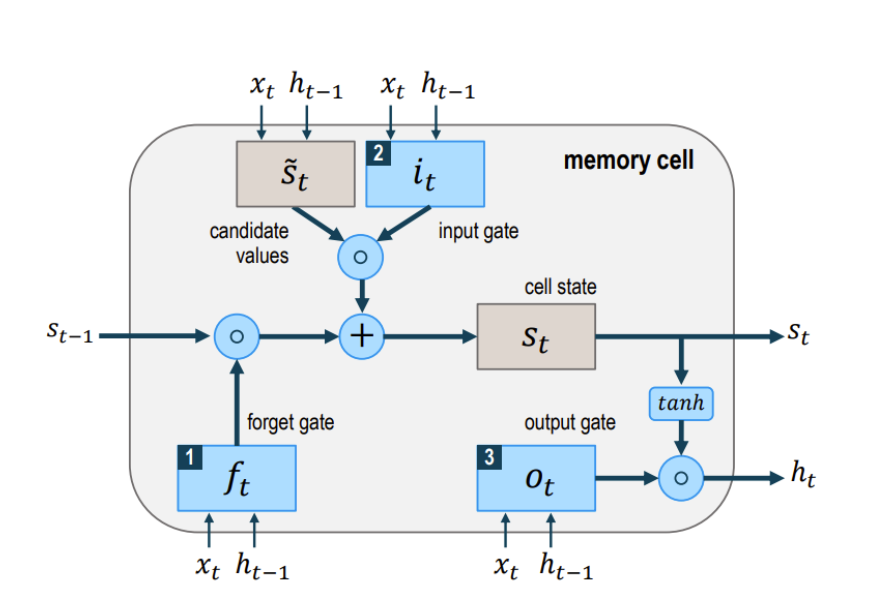
\includegraphics[width=0.7\textwidth]{figures/sodo.png}
    \caption{Sơ đồ biểu diễn kiến trúc bên trong của một tế bào LSTM}
\end{figure}

\subsubsection{Kiến trúc bên trong LSTM}
Bước đầu tiên của LSTM là quyết định xem thông tin nào cần bỏ đi từ trạng thái tế bào. Quyết định sẽ được  tầng sigmoid đưa ra hay còn gọi là tầng cổng quên (forget gate layer). Nó lấy đầu vào là $h_{t-1}$ và $x_t$  rồi đưa ra kết quả nằm trong khoảng $[0, 1]$ cho mỗi giá trị trong trạng thái tế bào $C_{t-1}$. Đẩu ra là $0$ chỉ rằng toàn bộ thông tin sẽ bị bỏ đi, còn $1$ thể hiện rằng nó giữ toàn bộ thông tin lại.\\

\begin{figure}[H]
    \centering
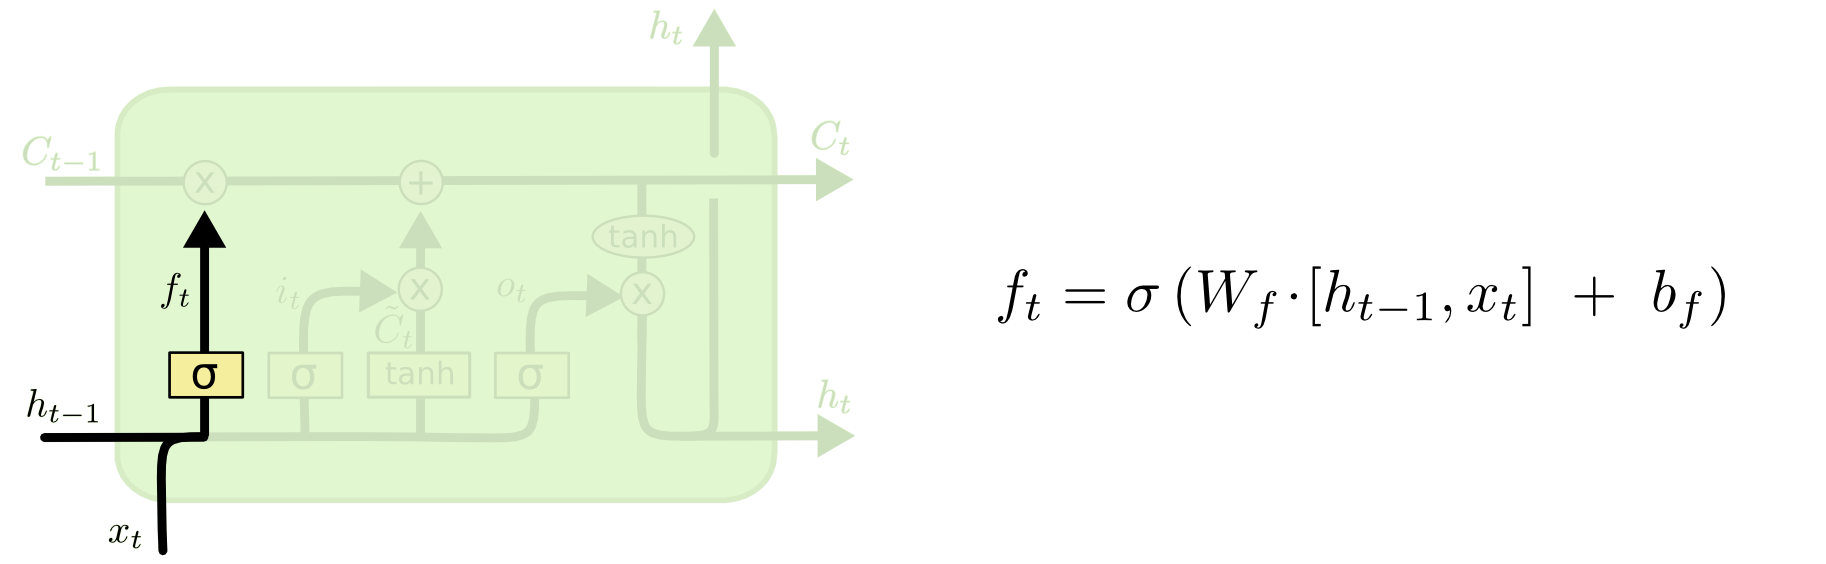
\includegraphics[width=0.9\textwidth]{figures/LSTM3-focus-f.png}
    \captionof{figure}[Tầng cổng quên]{Tầng cổng quên.}
\end{figure}
\par
Bước tiếp theo là quyết định xem thông tin mới nào ta sẽ lưu vào trạng thái tế bào. Việc này gồm 2 phần. Đầu tiên là sử dụng một tầng sigmoid - tầng cổng vào (input gate layer) để chọn giá trị cập nhật. Sau đó là tầng $tanh$ sẽ tạo ra một vector giá trị mới $\tilde{C_t}$ mục đích là thêm vào cho trạng thái. Trong bước kế tiếp ta sẽ kết hợp 2 giá trị trên với nhau nhằm mục đích tạo ra một cập nhật trang thái. \\
\begin{figure}[H]
    \centering
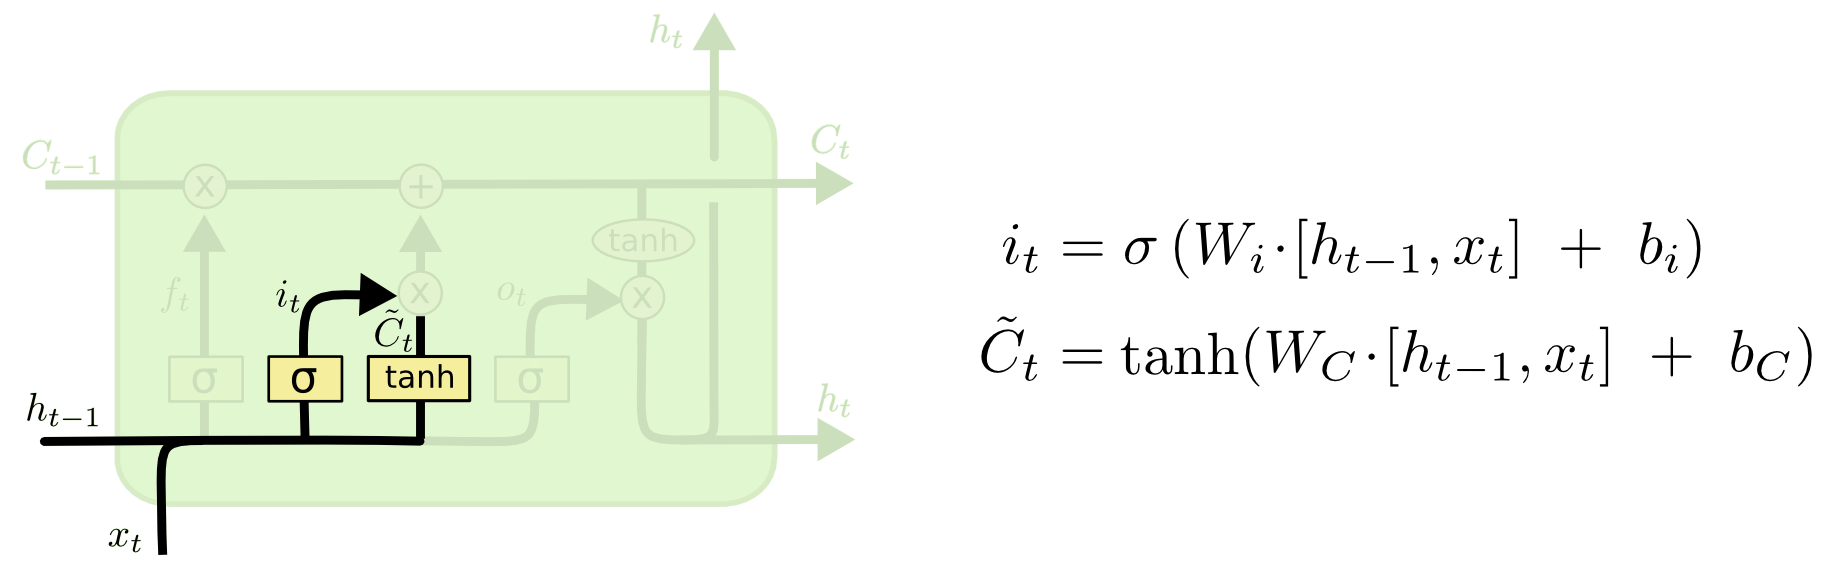
\includegraphics[width=0.9\textwidth]{figures/LSTM3-focus-i.png}
    \captionof{figure}[Tầng cổng vào]{Tầng cổng vào.}
\end{figure}

\par
Giờ là lúc cập nhập trạng thái tế bào cũ $C_{t-1}$  thành trạng thái mới $C_t$. Trong các bước trước đó đã quyết định các việc cần làm, nên bây giờ chỉ cần thực hiện.\\
Nhận trạng thái trước với $f_t$ để loại bỏ được những thông tin đã quyết định quên. Sau đó cộng thêm $i_t*\tilde{C_t}$. Trạng thái mơi thu được này phụ thuộc vào việc ta quyết định cập nhập mỗi giá trị trạng thái ra sao.\\
\begin{figure}[H]
\centering
	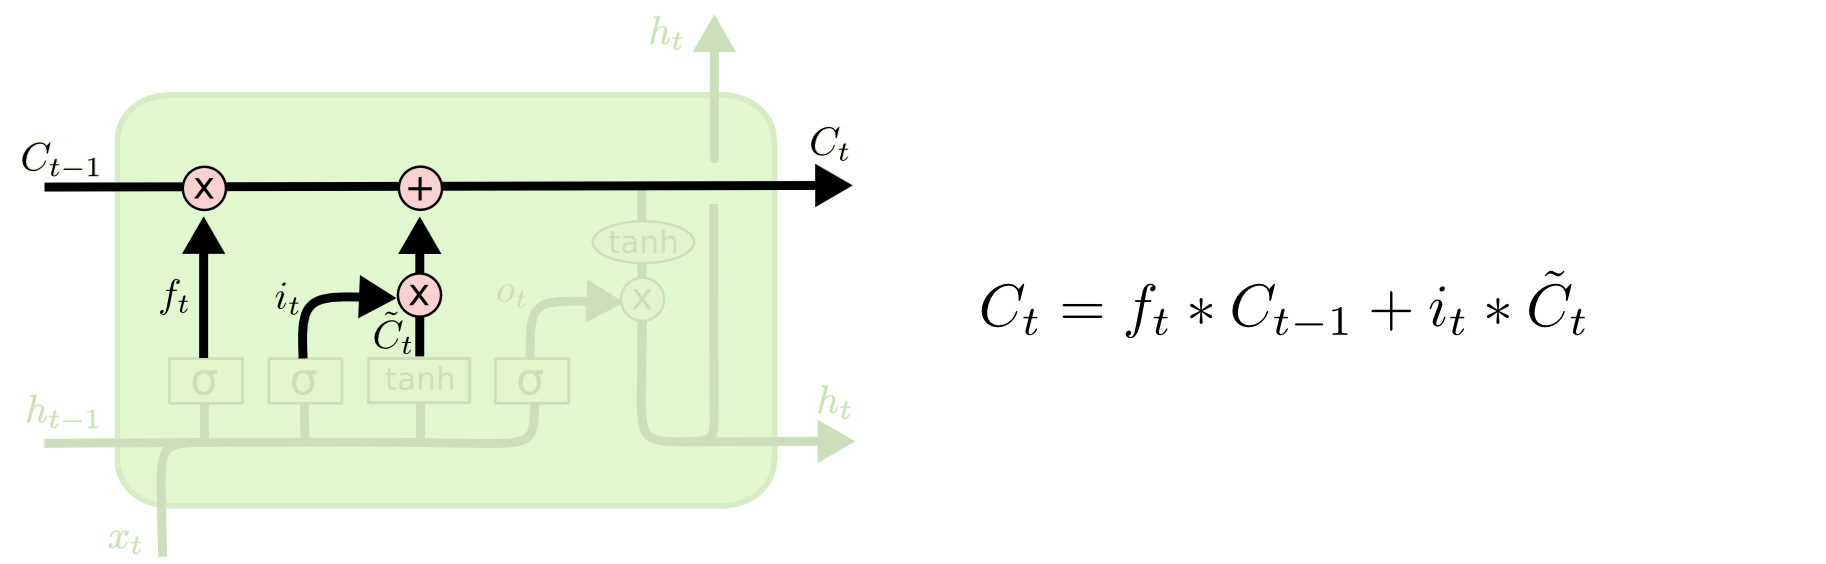
\includegraphics[width=0.9\textwidth]{figures/LSTM3-focus-C.png}
	\captionof{figure}[Cập nhật trạng thái tế bào]{Cập nhật trạng thái tế bào.}
\end{figure}

\par
Cuối cùng, ta cần xem xem đầu ra mong muốn là gì. Giá trị đầu ra sẽ dựa vào trạng thái tế bào và sẽ được tiếp tục sàng lọc. Trước tiên, ta chạy một tầng $sigmoid$ để chọn phần nào của trạng thái tế bào ta muốn xuất ra. Sau đó, ta đưa nó trạng thái tế bảo qua một hàm $tanh$ để co giá trị nó về khoảng $[-1, 1]$, và nhân nó với đầu ra của cổng sigmoid để được giá trị đầu ra ta mong muốn.
\begin{figure}[H]
\centering
	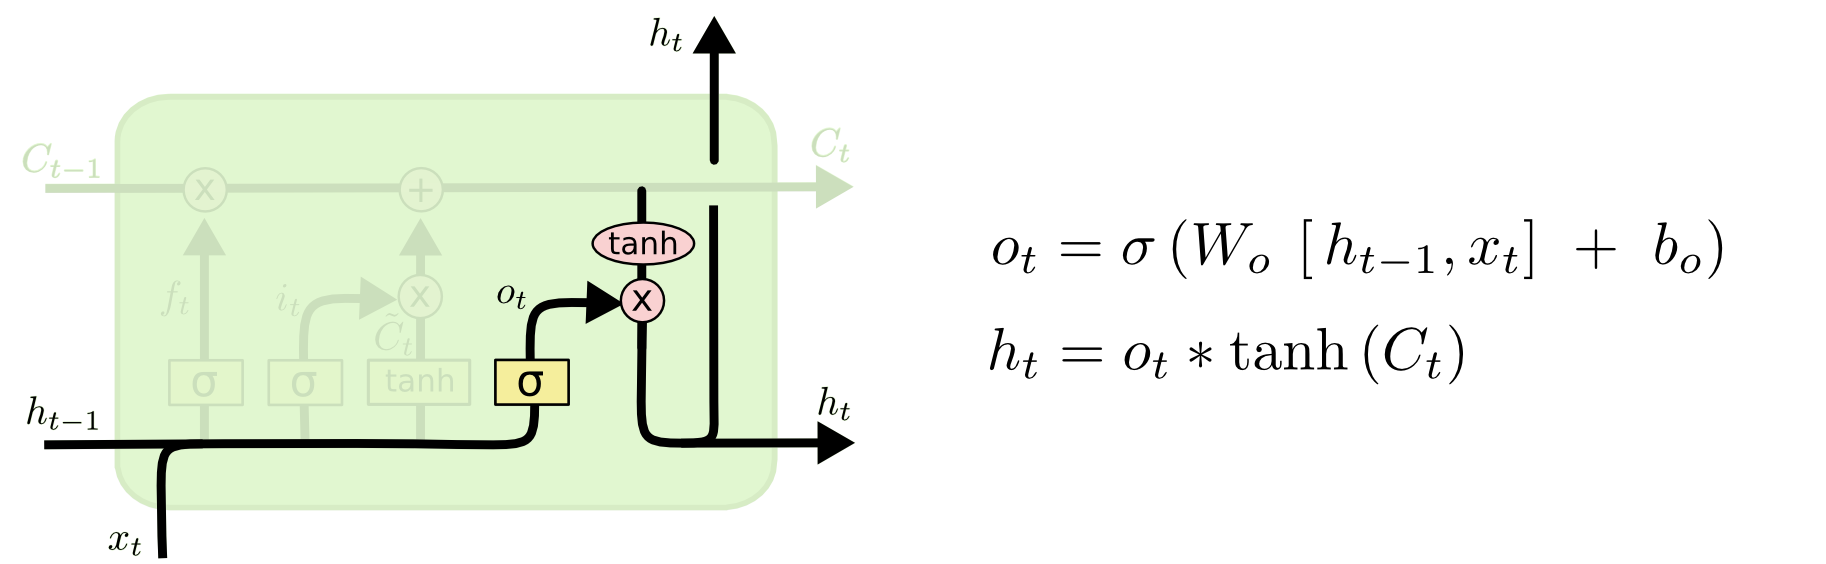
\includegraphics[width=0.9\textwidth]{figures/LSTM3-focus-o.png}
	\captionof{figure}[Cổng ra]{Cổng ra.}
\end{figure}

\section{VARMAX}
\subsection{Giới thiệu mô hình VARMAX}
Mô hình tự hồi quy trung bình trượt véc tơ với các biến hồi quy ngoại sinh (VARMAX). Đường tự hồi quy trung bình trượt véc tơ với các biến hồi quy ngoại sinh (VARMAX) là một phần mở rộng của mô hình VARMA cũng bao gồm mô hình hóa các biến ngoại sinh. Nó là phiên bản đa biến của phương pháp ARMAX.

Các biến ngoại sinh còn được gọi là đồng biến và có thể được coi là các chuỗi đầu vào song song có các quan sát ở các bước đồng thời với chuỗi ban đầu. (Các) chuỗi chính được gọi là dữ liệu nội sinh để đối chiếu nó với (các) chuỗi ngoại sinh. Các quan sát đối với các biến ngoại sinh được đưa trực tiếp vào mô hình tại mỗi bước thời gian và không được mô hình hóa theo cách giống như chuỗi nội sinh chính (ví dụ như quy trình AR, MA, v.v.).

Mô hình VARMAX là một mô hình phù hợp cho chuỗi thời gian đa biến. Nó thêm thành phần trung bình cộng vào mô hình VAR và có thể cho phép các biến ngoại sinh. Bởi vậy, mô hình VARMAX gồm các thành phần:
\begin{itemize}
    \item \textbf{VAR (Vector Autoregression):} thành phần tự hồi quy bao gồm tập hợp các độ trễ của biến hiện tại.
    \item \textbf{MA (Moving Average):} được hiểu là quá trình thay đổi hoặc dịch chuyển giá trị trung bình của một chuỗi theo thời gian.
    \item \textbf{X (Exogenous variable):} sử dụng các biến ngoại sinh.
\end{itemize}
Mô hình này có thể phù hợp với các quy trình phức tạp hơn nhiều mô hình chuỗi thời gian khác. Tuy nhiên, nó cũng có nhược điểm: thời gian train tương đối dài so với các mô hình đơn giản hơn và cần một lượng dữ liệu tương đối lớn để ước tính chính xác.

\subsection{Mô hình VARMAX(p,q)}
Mô hình toán học của VARMAX được định nghĩa như sau:
Công thức tổng quát cho mô hình VARMAX:
        $$X_t = \delta_t - \Sigma_{i=0}^p\phi_i X_{t-i} + \varepsilon_t + \Sigma_{i=1}^q \theta_i \varepsilon_{t-i}$$
        hay $\phi(B)X_t = \delta_t + \theta(B)\varepsilon_t$ \\
        tại $\phi(B) = I_k - \Sigma^p_{i=1}\phi_i B^i$, $\theta(B)=I_k-\Sigma^q_{i=1}\theta_i B^i$ \\
        và $\delta_t$ có thể là một hằng số xác định (biến ngoại sinh).


Các thành phần của VARMAX:
\begin{itemize}
		\item Auto regression: Kí hiệu là AR. Đây là thành phần tự hồi quy bao	gồm tập hợp các độ trễ của biến hiện tại. Mô hình AR có thể được biểu diễn như sau:\par
		\begin{equation}
		    y_{t}=c+\phi_{1}y_{t-1}+\epsilon_{t}
		\end{equation}
		Trong đó: $y_t$ là giá trị tại thời gian t, c là hằng số, $\Phi_1$ là hệ số còn $\epsilon_t$ là nhiễu trắng với $\epsilon_t \sim N(0, \sigma^2)$.
		
		Độ trễ bậc p chính là giá trị lùi về quá khứ p bước thời gian của chuỗi. Độ trễ dài hoặc ngắn trong quá trình AR phụ thuộc vào tham số trễ p. Mô hình AR(p) của chuỗi $y_t$ được biểu diễn như sau:\par
		\begin{equation}
		    y_{t}=c+\phi_{1}y_{t-1}+\phi_{2}y_{t-2}...+\phi_{p}y_{t-p}+\epsilon_{t}
		\end{equation}
		    hay\par
		\begin{equation}
		    y_{t}=c+\sum_{i=1}^{p}\phi_{i}y_{t-i}
		\end{equation}
		
		    Trong đó $\Phi_i$ là hệ số tương ứng của mỗi giá trị $y{_t-i}$.\par
		\item 	Moving average: Quá trình trung bình trượt được hiểu là quá trình dịch chuyển hoặc thay đổi giá trị trung bình của chuỗi theo thời gian. Do chuỗi của chúng ta được giả định là dừng nên quá trình thay đổi trung bình dường như là 1 chuỗi nhiễu trắng. Quá trình moving average sẽ tìm mối liên hệ về mặt tuyến tính giữa các phần tử ngẫu nhiên $\epsilon_t$ chuỗi này là 1 chuỗi nhiễu trắng có các tính chất:\par
		\begin{align}
		    E(\epsilon_{t})=0\label{hang1}\\
		    \sigma(\epsilon_{t})=\alpha	\label{hang2}\\
		     \rho(\epsilon_{t},\epsilon_{t-s)}=0, \forall  t\geq s\label{hang3}
		\end{align}
		Vế \eqref{hang1} có nghĩa rằng kì vọng của chuỗi dừng bằng 0 để đảm bảo chuỗi dừng không có sự thay đổi về trung bình theo thời gian. Vế \eqref{hang2} là phương sai của chuỗi không đổi. Do kì vọng và phương sai không đỏi nên chúng tagọi phân phối của nhiễu trắng là phân phối xác định và được kí hiệu $\epsilon_t \sim \mathcal{WN}(\ {0},\,\sigma^{2})$. Nhiễu trắng là một thành phần ngẫu nhiên thể hiện cho yếu tố không thể dự báo của model và không có tính quy luật. Quá trình trung bình trượt được biểu diễn theo nhiễu trắng như sau:\par
		\begin{equation}
		    MA(q)=\mu+\sum_{i=1}^{q}\theta_{i}\epsilon_{t-i}
		\end{equation}
	\end{itemize}

 \subsection{Cách xác định hệ số p, q}
 \subsubsection{Cách xác định hệ số p của AR}
     Để kiểm tra hệ số q của mô hình AR ta kiểm tra biểu đồ tự tương quan 1 phần (PACF). \par
     Tự tương quan một phần có thể được hình dung như mối tương quan giữa chuỗi và độ trễ của nó, sau khi loại trừ các đóng góp từ độ trễ trung gian. Vì vậy, PACF truyền tải mối tương quan thuần túy giữa độ trễ và chuỗi. Bằng cách đó, ta sẽ biết liệu độ trễ đó có cần thiết trong điều kiện AR hay không.\par
     Bất kỳ sự tự tương quan nào trong một chuỗi dừng đều có thể được điều chỉnh bằng cách thêm đủ các thuật ngữ AR. Vì vậy, ban đầu ta coi thứ tự của số hạng AR bằng với càng nhiều độ trễ vượt qua giới hạn ý nghĩa trong biểu đồ PACF.\par
\begin{figure}[H]
    \centering
    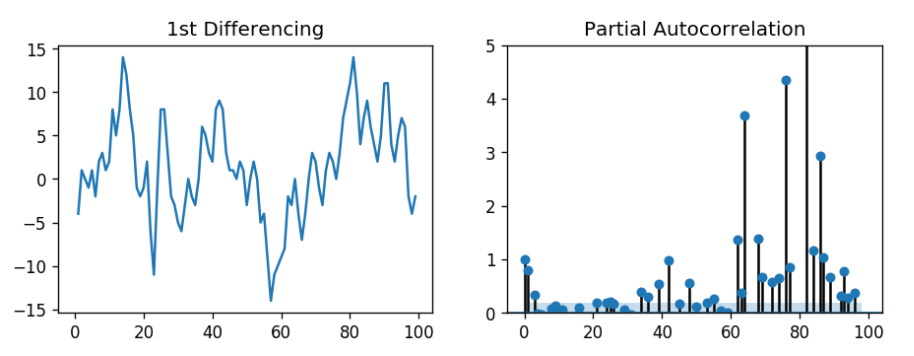
\includegraphics[scale=0.8]{figures/PACF.png}
    \caption{Ví dụ cách xác định p}
\end{figure}     
     Có thể quan sát thấy rằng độ trễ PACF bằng 1 là khá đáng kể vì nằm trên đường ý nghĩa (vùng màu xanh lam). Vì vậy ta chọn p bằng 1.
\subsubsection{Cách xác định hệ số q của MA}
     Cũng giống như cách xem xét biểu đồ PACF cho hệ số của AR, chúng ta có thể xem biểu đồ ACF để biết hệ số của MA.\par
\begin{figure}[H]
    \centering
    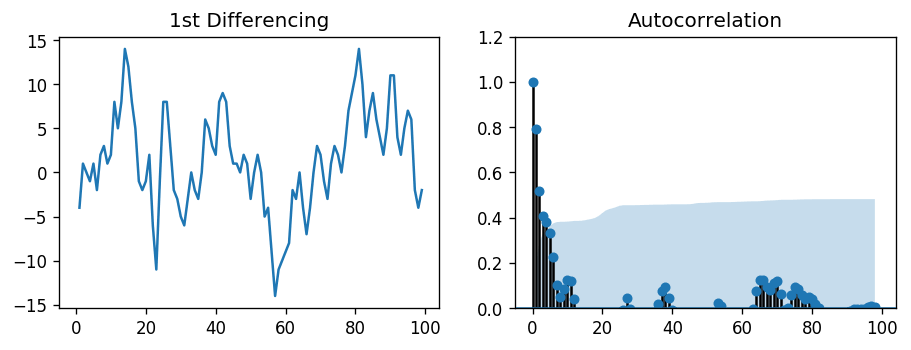
\includegraphics[scale=0.45]{figures/ACF.png}
    \caption{Ví dụ cách xác định q}
\end{figure}
     Biểu đồ ACF cho ta biết cần phải thực hiện quá trình MA bao nhiêu lần để loại bỏ sự tự tương quan trong chuỗi thời gian dừng. Ở đây ta thấy nhiều là nằm trên đường ý nghĩa, ta có thể chọn giá trị q là 1 hoặc 2.
\subsection{Ước lượng tham số mô hình sử dụng thuật toán đổi mới}
     Giả sử ta có một chuỗi ARMA(p,q) dừng với các quan sát $X_{t}, t=1,2,...,N$. Mô hình \text{ARMA(p,q)} đưa ra bởi $X_t$:\par
     \begin{equation}
         \phi(B)X_{t}=\theta(B)Z_{t}
     \end{equation}\par
     Với $\phi(B)$ và $\theta(B)$ là các đa thức bậc p và q\par
     \begin{equation}
         \phi(B)=1-\phi_{1}B-...-\phi_{p}B^{p}
     \end{equation}\par
     và\par
     \begin{equation}\label{ARMA(1)}
         \theta(B)=1+\theta_{1}B+...\theta_{q}B^{q}
     \end{equation}\par
     Với B là toán tử lùi xác định bởi ($B^{j}X_{t}=X_{t-j}, B^{j}Z_{t}=Z_{t-j}, j=0,\pm1,...$), $Z_{t}$ là chuỗi nhiễu trắng với kỳ vọng bằng 0 và phương sai là $\sigma^{2}$.\par
     \begin{equation}\label{ARMA(2)}
         X_{t}-\phi_{1}X_{t-1}-...-\phi_{p}X_{t-p}=Z_{t}+\theta_{1}Z_{t-1}+...\theta_{q}Z_{t-q}
     \end{equation}\par
     Khi p=0 thì biểu thức \eqref{ARMA(2)} là một chuỗi MA(q) còn nếu q=0 thì biểu thức \eqref{ARMA(2)} là một chuỗi AR(p). Brockwell và Davis (1987) đã đưa ra một thuật toán để ước tính các tham số AR và MA cho một mô hình ARMA (p, q). Theo đó, với hàm tự tương phương sai đã biết(ACVF) $\gamma(.)$ thì các ước lượng đổi mới $\theta_{1,1},\theta_{2,2},\theta_{2,1},\theta_{3,3},\theta_{3,2},...$ có thể có được theo các biểu thức:\par
     \begin{align}
         V_{0}=\gamma(0)\label{ARMA(3)}\\
         \theta_{m,m-k}=V_{k}^{-1}[\gamma(m-k)-\sum_{j=0}^{k-1}\theta_{m,m-j}]\label{ARMA(4)}\\
         V_{m}=\gamma(0)-\sum_{j=0}^{m-1}\theta_{m,m-j}V_{j}\label{ARMA(5)}
     \end{align}\par
     Nếu quá trình được cho bởi phương trình \eqref{ARMA(1)} là khả nghịch, thì nó có thể được biểu diễn dưới dạng:\par
     \begin{equation}
         X_t=\sum_{j=0}^{\infty}\psi_{j} W_{t-j}\label{ARMA(6)}
     \end{equation}\par
     Biểu thức \eqref{ARMA(1)} và \eqref{ARMA(6)} có thể được biểu diễn:\par
     \begin{align}
         \psi_{0}=1\label{ARMA(7)}\\
         \psi_{j}=\theta_{j}+\sum_{i=1}^{min(j,p)}\theta_{i}\psi_{j-1}, j=1,2,...\label{ARMA(8)}
     \end{align}\par
     Theo quy ước ta có $\theta_{j}=0$ với j > q và $\phi_{i}=0$ với i > p của chuỗi ARMA(p,q). Brockwell và Davis (1987) còn chứng minh thêm rằng $\psi_{j}\longrightarrow\theta_{m,j}$. Do đó biểu thức\eqref{ARMA(8)} được viết dưới dạng:\par
     \begin{equation}
         \theta_{m,j}=\theta_{j}+\sum_{i=1}^{min(j,p)}\phi_{i}\theta_{m,j-1},j=1,2,...p+q\label{ARMA(9)}
     \end{equation}\par
     Với j=q+1, q+2,...q+p trong biểu thức \eqref{ARMA(9)} một hệ p phương trình có thể được tạo ra và chúng có dạng:\par
     \begin{equation}\label{ARMA(10)}
         \begin{bmatrix}
               \theta_{m,q+1}\\
               \theta_{m,q+2}\\
               \vdots\\
               \theta_{m,q+p}
         \end{bmatrix}
         =\
         \begin{bmatrix}
               \theta_{m,q}&\theta_{m,q-1}&\cdots&\theta_{m,q+1-p}\\
               \theta_{m,q+1}&\theta_{m,q}&\cdots&\theta_{m,q+2-p}\\
               \vdots&\vdots&\cdots&\vdots\\
               \theta_{m,q+p-1}&\theta_{m,q+p-2}&\cdots&\theta_{m,q}
         \end{bmatrix}
         \begin{bmatrix}
               \phi_1\\
               \phi_2\\
               \vdots\\
               \phi_p
         \end{bmatrix}
     \end{equation}\par
      Các giá trị của ($\phi_{1},\phi_{2},...\phi_{p}$) có thể được xác định bởi biểu thức\eqref{ARMA(10)}. Từ biểu thức \eqref{ARMA(9)}, $\theta_{j}$ có thể được xác định bởi phương trình:\par
      \begin{equation}\label{ARMA(11)}
          \theta_{j}=\theta_{m,j}-\sum_{i=1}^{min(j,p)}\phi_{i}\theta_{m,j-i},j=1,2,...q
      \end{equation}\par
      Các kỹ thuật ở trên có thể được sử dụng để xác định tham số của AR và MA $\phi_{1},\phi_{2},...\phi_{p},\theta_{1},\theta_{2},...,\theta_{q}$ trong mô hình ARMA.
	\chapter{CÀI ĐẶT VÀ ĐÁNH GIÁ KẾT QUẢ}
\section{Mô tả dữ liệu}
%chèn plot giá của tập dữ liệu theo thời gian, nêu rõ thời gian thu thập, nguồn thu thập, kích thước dữ liệu, tỉ lệ chia tập train, val, test
Để thực hiện dự đoán trên hai mô hình LSTM và VARMAX, chúng em sẽ thực nghiệm trên dữ liệu về chỉ số môi trường không khí.
\begin{itemize}
    \item Nguồn thu thập: Được cung cấp bởi giảng viên bộ môn
    \item Thời gian của dữ liệu: 142 ngày từ 7:00 14/4/2019 đến 6:00 5/9/2019 tính theo từng giờ.
    \item Kích thước dữ liệu: 556KB
    \item Giá trị cần dự đoán: mô hình dự đoán tất cả các giá trị trong bộ dữ liệu
    
\end{itemize}
\begin{figure}[H]
    \centering
    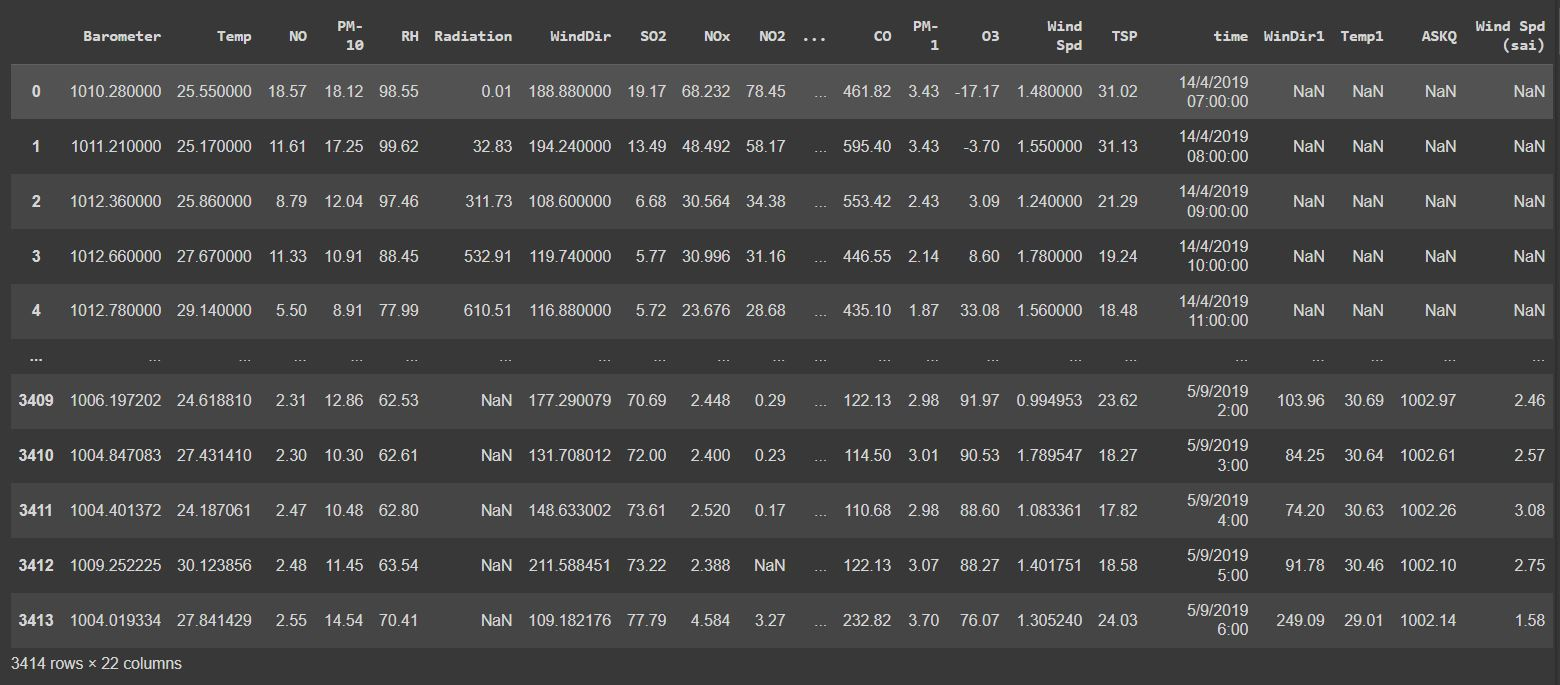
\includegraphics[width=.95\textwidth]{figures/data.jpg}
    \caption[Dữ liệu môi trường không khí từ  7:00 14/4/2019 đến 6:00 5/9/2019]{Dữ liệu môi trường không khí từ  7:00 14/4/2019 đến 6:00 5/9/2019}
\end{figure}


Mô tả chi tiết tên các cột :
\begin{itemize}
    \item Barometer: hay còn được gọi với thuật ngữ quen thuộc là áp kế, là tính năng dùng để đo áp suất khí quyển ở vị trí hiện tại của đồng hồ. Đơn vị đo áp suất phổ biến hiện nay là (hPa) = hectopascal, ngoài ra còn 2 đơn vị được sử dụng nhiều là kilopascal (kPa) và atmosphere (atm).
    \item Temp : là nhiệt độ đơn vị độ C
    \item NO : Nitơ monoxide, hay còn gọi là nitric oxide (công thức hóa học: NO) là chất khí không màu, không bền trong không khí vì bị oxy oxy hóa ở nhiệt độ thường tạo ra nitơ dioxide là chất khí màu nâu đỏ. NO được tạo ra từ năng lượng sấm sét
    \item NO2 : Nitrogen dioxide (NO 2 ) là một chất góp phần chính trong việc hình thành sương mù và là tiền thân của nhiều chất ô nhiễm thứ cấp có hại, bao gồm ozone và các chất dạng hạt. Nó phản ứng mạnh với các hóa chất khác và là một chất oxy hóa mạnh. Nitơ đioxit là một chất khí có màu đỏ cam đậm.
    \item NOx : là chất gây ô nhiễm chính trong khí quyển, là tác nhân của mưa axit, sương khói quang hóa và tích tụ ozone. Các oxit chủ yếu là nitơ monoxit (NO) và nitơ dioxit (NO2) cả hai đều ăn mòn và nguy hiểm cho sức khỏe.
    \item PM-10 : PM-10 là những hạt rất nhỏ được tìm thấy trong bụi và khói . Chúng có đường kính 10 micromet (0,01 mm) hoặc nhỏ hơn. Các hạt PM-10 là một chất gây ô nhiễm không khí phổ biến.
    \item RH : Độ ẩm tương đối (RH) là thước đo lượng hơi nước trong hỗn hợp nước-không khí so với lượng tối đa có thể. RH là tỷ lệ giữa tỷ lệ độ ẩm của hỗn hợp nước-không khí cụ thể so với tỷ lệ độ ẩm bão hòa ở một nhiệt độ nhất định.
    \item Radition : Bức xạ khí quyển là dòng năng lượng điện từ giữa mặt trời và bề mặt trái đất khi nó bị ảnh hưởng bởi các đám mây và khí trong bầu khí quyển của trái đất. Nó bao gồm cả bức xạ mặt trời (ánh sáng mặt trời) và bức xạ nhiệt.
    \item SO2 : Lưu huỳnh dioxit là chất gây ô nhiễm không khí phản ứng, không màu, có mùi nồng . Loại khí này có thể là mối đe dọa đối với sức khỏe con người, sức khỏe động vật và đời sống thực vật. Các nguồn phát thải sulfur dioxide chính là từ quá trình đốt cháy nhiên liệu hóa thạch và hoạt động núi lửa tự nhiên.
    \item PM-2-5: là những hạt bụi li ti có trong không khí với kích thước 2,5 micron trở xuống (so với sợi tóc con người thì nó nhỏ hơn khoảng 30 lần). Bụi mịn pm2. 5 được hình thành từ các chất như nitơ, carbon và các hợp chất kim loại khác. Nó chất gây ô nhiễm không khí gây lo ngại cho sức khỏe của mọi người khi nồng độ trong không khí cao.
    \item CO: Cacbon monoxit là một chất khí vô hình, không hề có màu sắc, vô vị, không hề có mùi, và nó là một chất độc nguy hiểm với độc tính cao. Nó là sản phẩm chính của quá trình đốt cháy nhiên liệu trong môi trường không đủ oxy.
    \item Là những hạt bụi dạng lỏng, hoặc rắn trôi nổi ngoài không khí. PM1 được coi là đặc biệt nguy hiểm do kích thước cực nhỏ của nó. Đường kính của hạt càng nhỏ thì nó càng gây ra nhiều tác hại.
    \item O3 : là một chất khí màu xanh lam nhạt, có mùi hăng đặc biệt. Nó là một dạng thù hình của oxy kém bền hơn nhiều so với dạng nguyên tử O2, bị phá vỡ trong bầu khí quyển thấp hơn thành O2.
    \item Wind Spd : Tốc độ gió hay còn gọi là tốc độ luồng gió, là một đại lượng khí quyển cơ bản do không khí di chuyển từ nơi có áp suất cao đến áp suất thấp.
    \item TSP: Tổng bụi lơ lửng (TSP) là tổng các hạt bụi có đường kính khí động học nhỏ hơn hoặc bằng 100 micromet. 
\end{itemize}

\newpage
\section{Xử lý dữ liệu}
\noindent \textbf{Vấn đề của bộ dữ liệu} : có khá nhiều dữ liệu bị khuyết thiếu.
\begin{figure}[H]
    \centering
    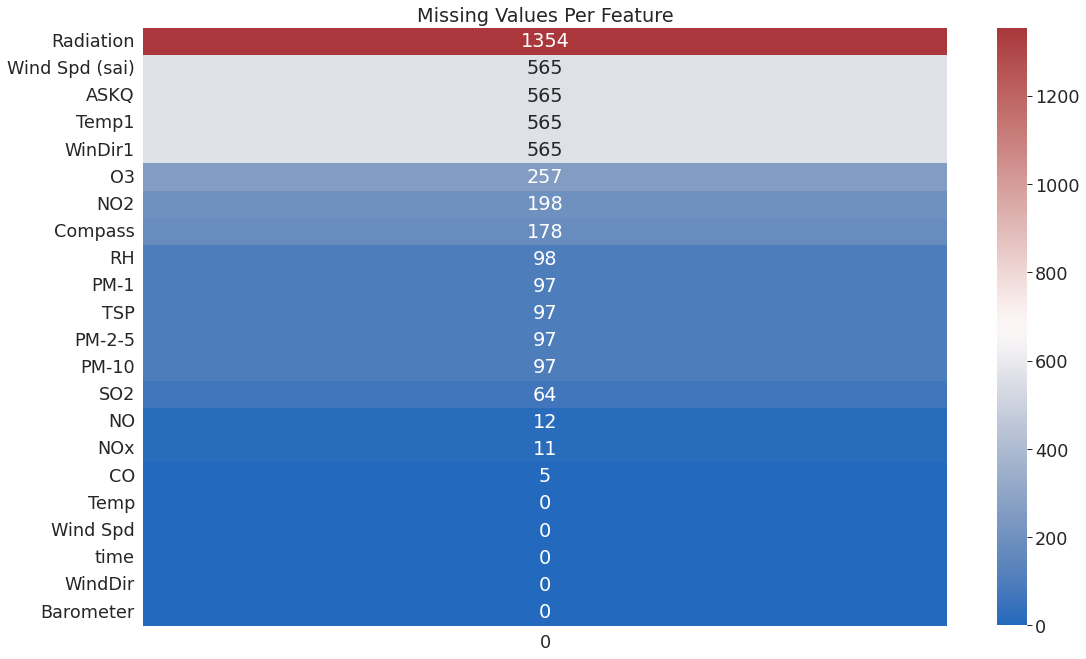
\includegraphics[width=.93\textwidth]{figures/missing.png}
    \caption[Số lượng dữ liệu khuyết thiếu của từng cột]{Số lượng dữ  liệu khuyết thiếu của từng cột}
\end{figure}

\begin{figure}[H]
    \centering
    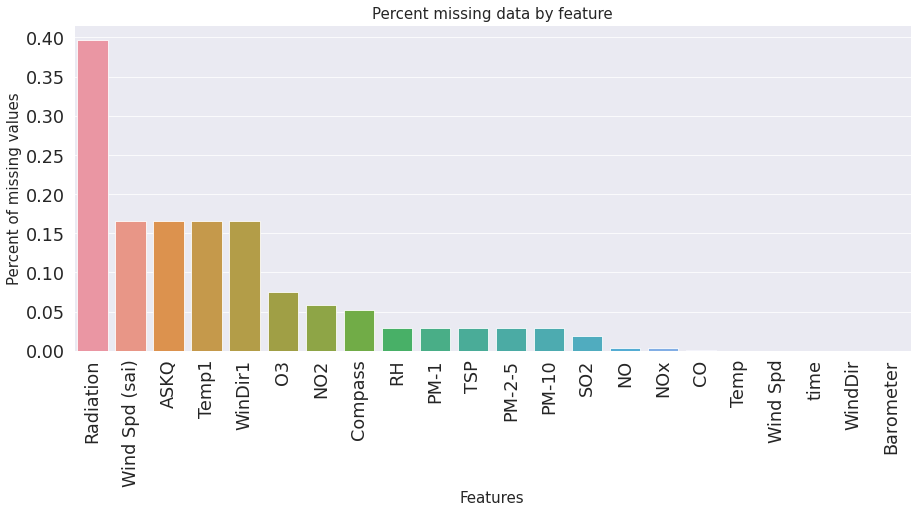
\includegraphics[width=.95\textwidth]{figures/missing2.png}
    \caption[Tỷ lệ dữ liệu khuyết thiếu của từng cột]{Tỷ lệ dữ liệu khuyết thiếu của từng cột}
\end{figure}

Nhận thấy tỷ lệ dữ liệu khuyết thiếu của từng cột cũng không cao lắm nên có thể giữ lại và sẽ sử dụng Linear-Regression để dự đoán các giá trị còn thiếu như sau:
\begin{lstlisting}
from sklearn.linear_model import LinearRegression
linreg = LinearRegression()

lst = ['CO', 'NOx','NO','SO2','PM-10','PM-2-5','TSP','PM-1','RH','Compass', 'NO2','O3','WinDir1','Temp1','ASKQ','Wind Spd (sai)','Radiation']
data = df[['Barometer','Wind Spd','Temp','WindDir']]
for a in lst:
    data = pd.concat([data, df[a]], axis=1)
    x_train = data[data[a].notnull()].drop(columns=a)
    y_train = data[data[a].notnull()][a]
    x_test = data[data[a].isnull()].drop(columns=a)
    y_test = data[data[a].isnull()][a]
    linreg.fit(x_train, y_train)
    predicted = linreg.predict(x_test)
    data[a][data[a].isnull()] = predicted
    df[a][df[a].isnull()] = predicted
    print("done")
\end{lstlisting}

\noindent Trong đó:
\begin{itemize}
    \item \textbf{lst} là 1 mảng chứa tên các cột bị thiếu dữ liệu được sắp xếp theo số lượng tăng dần.
    \item \textbf{data} chứa các cột có đủ dữ liệu.
\end{itemize}

\noindent Thực hiện:
\begin{itemize}
    \item Ta sử dụng vòng lặp for để dự đoán các cột có số lượng dữ liệu bị thiếu ít hơn trước. 
    \item Trong vòng lặp for, ta thêm 1 cột khuyết thiếu dữ liệu vào \textbf{data}
    \item Chia dữ liệu thành tập train và test:
    \begin{itemize}
        \item train: chứa các dòng dữ liệu đầy đủ.
        \item test: chứa các dòng dữ liệu bị khuyết thiếu.
    \end{itemize}
    \item Sử dụng mô hình dự đoán Linear-Regression để đưa ra kết quả dự đoán của tập test và tiếp tục quá trình nếu còn thỏa mãn vòng lặp.
\end{itemize}
\newpage
\noindent Kết quả thu được:
\begin{figure}[H]
    \centering
    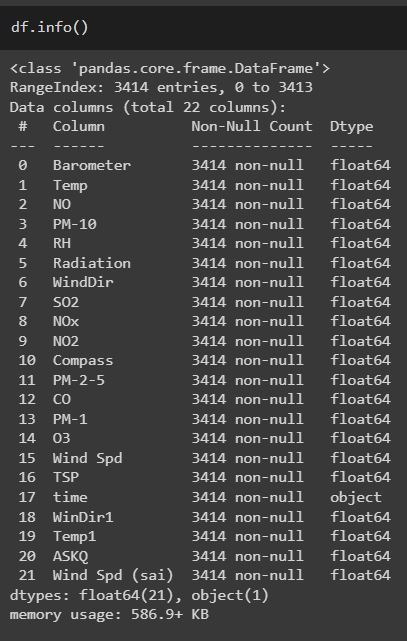
\includegraphics[width=.3\textwidth]{figures/info.jpg}
    \caption[Thông tin dữ liệu sau khi xử lý]{Thông tin dữ liệu sau khi xử lý}
\end{figure}

\begin{figure}[H]
    \centering
    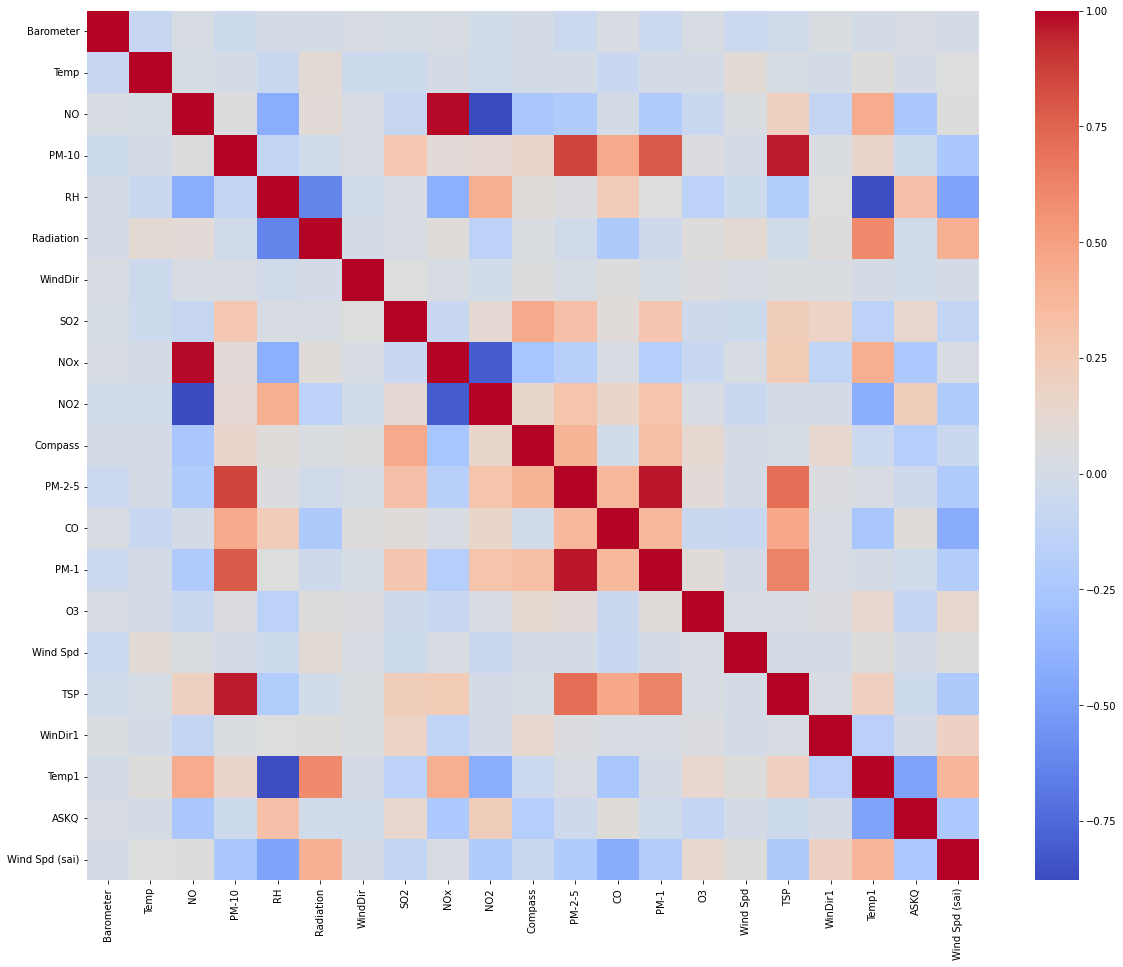
\includegraphics[width=.9\textwidth]{figures/matran.png}
    \caption[Heatmap]{Heatmap}
\end{figure}

\newpage
\begin{figure}[H]
    \centering
    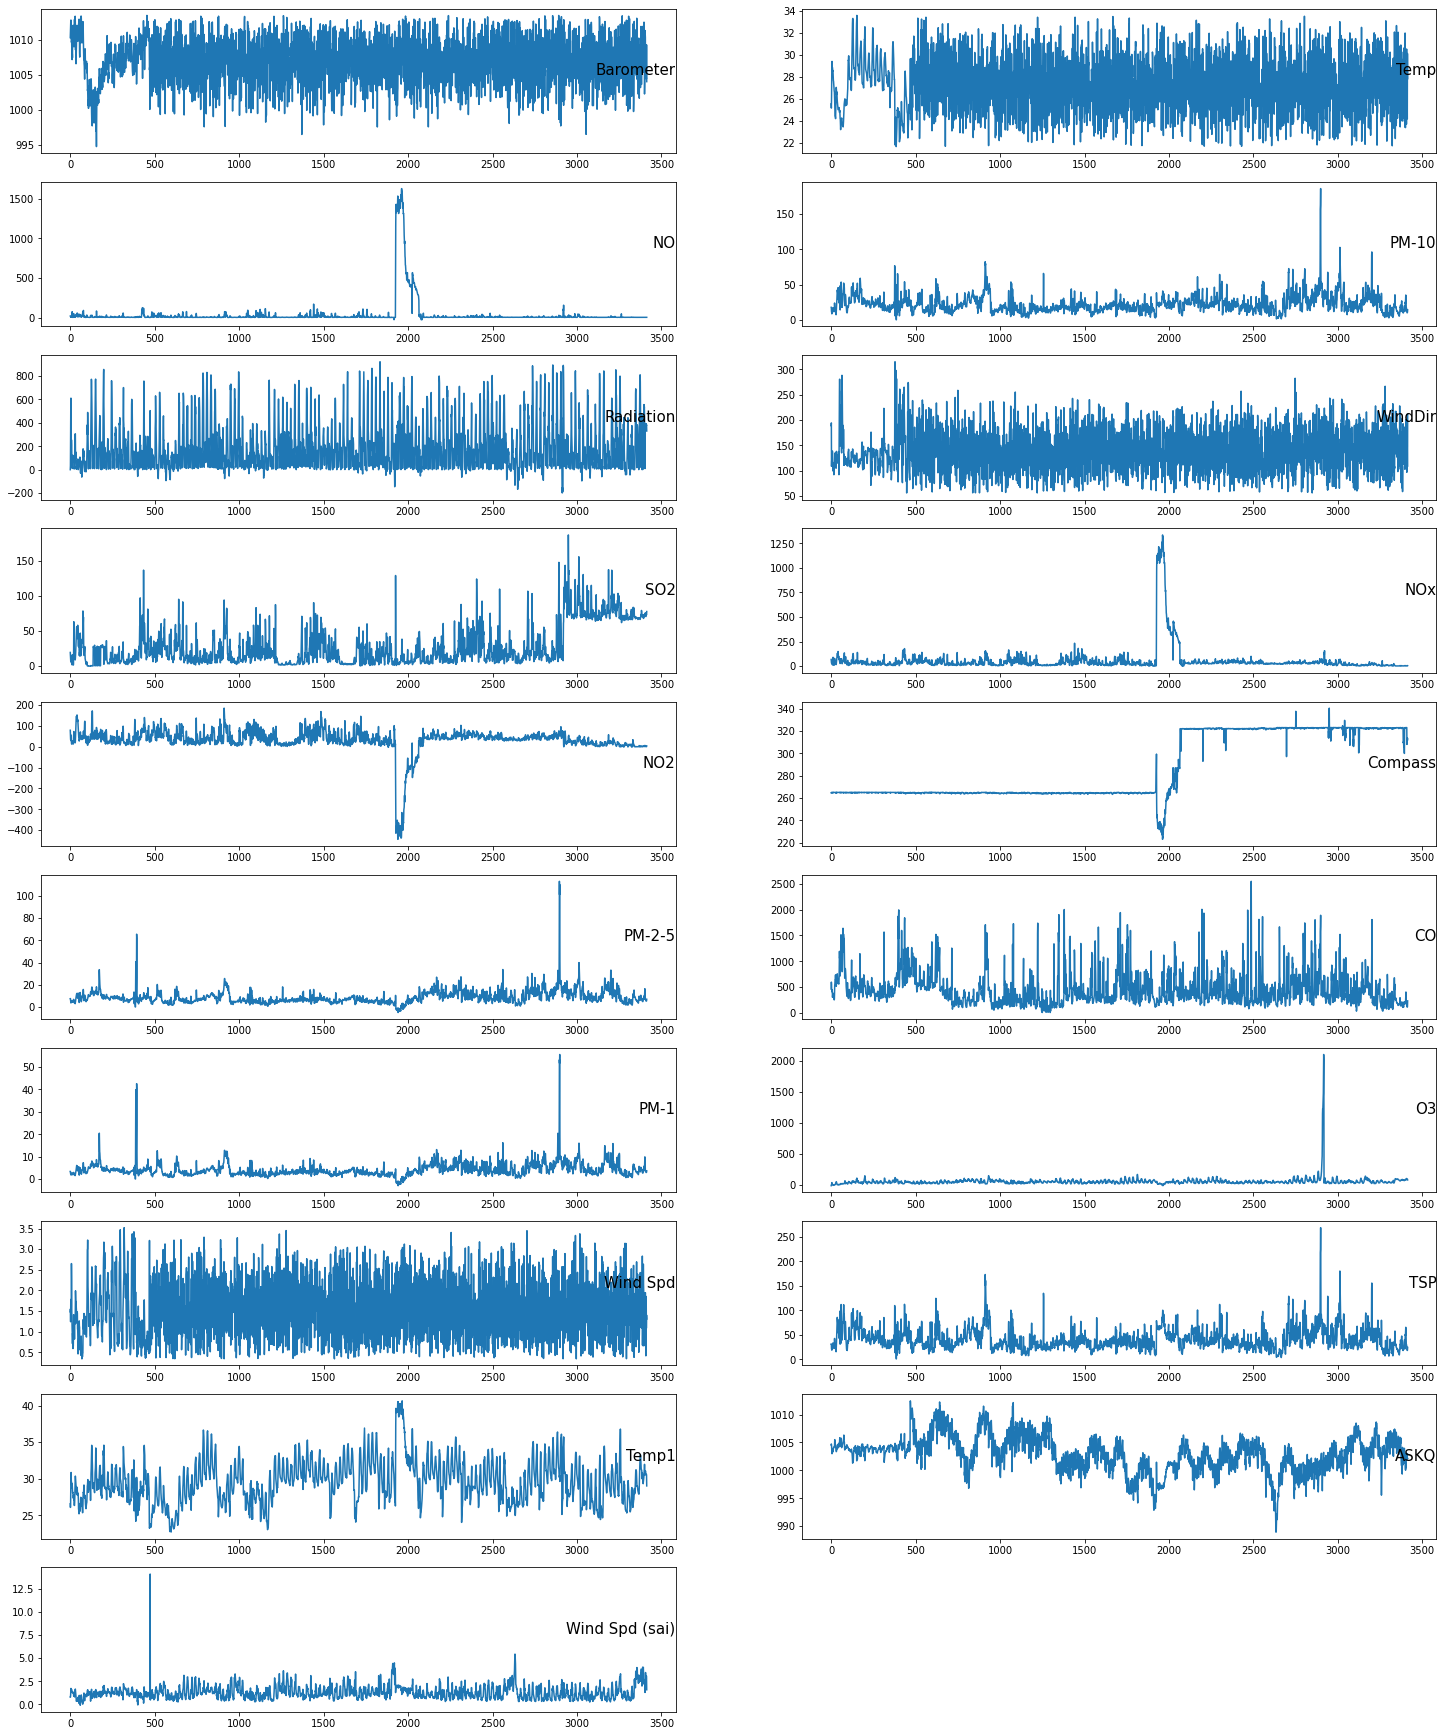
\includegraphics[width=.99\textwidth]{figures/trucquan.png}
    \caption[Trực quan hóa dữ liệu]{Trực quan hóa dữ liệu}
\end{figure}

\section{Tiêu chuẩn đánh giá mô hình}
%RMSE, MAE, MAPE
\subsection{Mean Squared Error (MSE)}
MSE được hiểu là giá trị sai số bình phương trung bình hoặc là lỗi bình phương trung bình. Nó đề cập đến giá trị trung bình của chênh lệch bình phương giữa tham số dự đoán và tham số quan sát được và có công thức như sau:
\begin{equation}
    \text{MSE} = \frac{1}{n}\sum_{i=1}^n(y_i - \hat{y_i})^2
\end{equation}
với $y_i$ là giá trị thực sự cần dự đoán, và $\hat{y}_i$ là giá trị mô hình dự đoán, $n$ là kích thước của dữ liệu cần dự đoán.


\subsection{Root Mean Squared Error (RMSE)}
RMSE là thước đo mức độ hiệu quả của mô hình của bạn. Nó thực hiện điều này bằng cách đo sự khác biệt giữa các giá trị dự đoán và giá trị thực tế . R-MSE càng nhỏ tức là sai số càng bé thì mức độ ước lượng cho thấy độ tin cậy của mô hình có thể đạt cao nhất và có công thức tính là:
\begin{equation}
    \text{RMSE} = \sqrt{\frac{1}{n}\sum_{i=1}^n(y_i - \hat{y_i})^2}
\end{equation}
với $y_i$ là giá trị thực sự cần dự đoán, và $\hat{y}_i$ là giá trị mô hình dự đoán, $n$ là kích thước của dữ liệu cần dự đoán.

\subsection{Sử dụng \textit{model.plot\_diagnostics()}}
\noindent Tạo lưới ô 2x2 chứa các kết quả đánh giá mô hình:
\begin{enumerate}
    \item Standardized residuals 
    \item Histogram plus estimated density 
    \item Normal Q-Q
    \item Correlogram
\end{enumerate}

\section{Kết quả}
%chèn plot so sánh kết quả ở tập train, tập test.
%ghi kết quả vào bảng sau
\subsection{Mô hình LSTM}
Đánh giá mô hình :
\begin{itemize}
    \item Loss: được tính bằng MSE, LOSS của mô hình sau khi huấn luyện qua 200 epoch
    \begin{figure}[H]
    \centering
    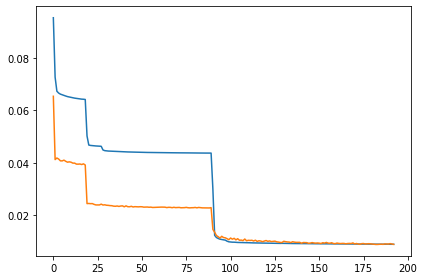
\includegraphics[width=.95\textwidth]{figures/LOSS_LSTM.png}
    \caption[LOSS của mô hình LSTM]{LOSS của mô hình LSTM}
    \end{figure}
    \item RMSE của mô hình sau khi huấn luyện qua 200 epoch:
    \begin{figure}[H]
    \centering
    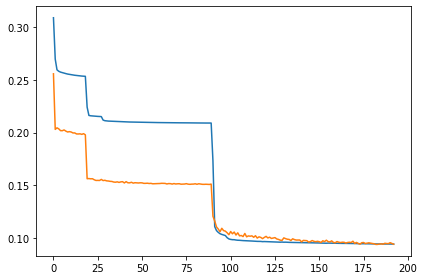
\includegraphics[width=.95\textwidth]{figures/RMSE_LSTM.png}
    \caption[RMSE của mô hình LSTM]{RMSE của mô hình LSTM}
\end{figure}

\end{itemize}
Kết quả dự đoán của mô hình với 48 giờ cuối của bộ dữ liệu so với giá trị thực trên tập dữ liệu:
    \begin{figure}[H]
    \centering
    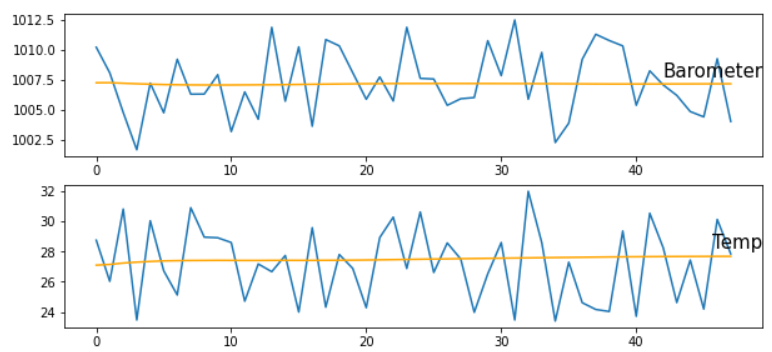
\includegraphics[width=1\textwidth]{figures/LSTM_test1.png}
    \caption[Barometer và Temp]{Barometer và Temp}
\end{figure}
\newpage
\begin{figure}[H]
    \centering
    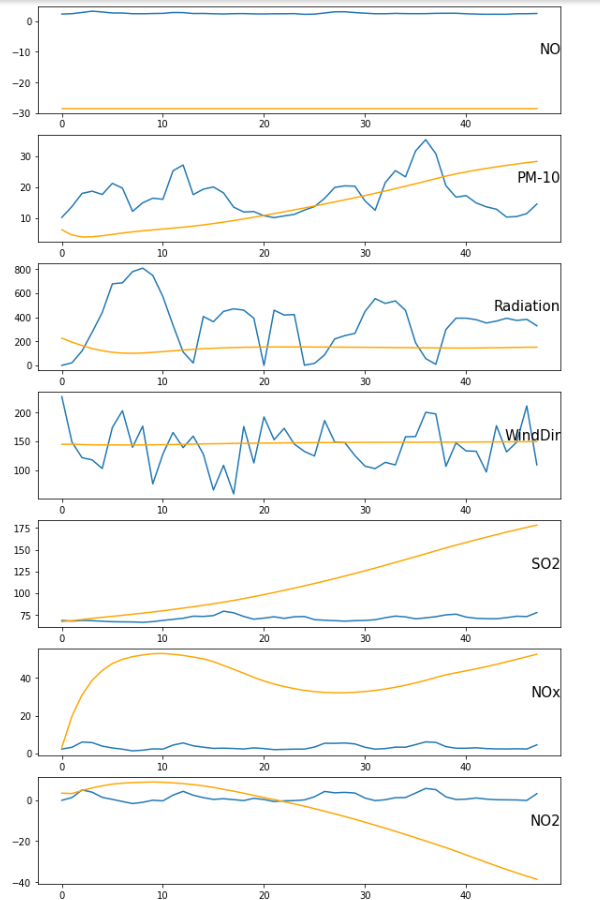
\includegraphics[width=.95\textwidth]{figures/LSTM_test3.png}
    \caption[NO, PM-10, Radition, WindDir và SO2]{NO, PM-10, Radition, WindDir, SO2, NOx và NO2}
\end{figure}
\newpage
\begin{figure}[H]
    \centering
    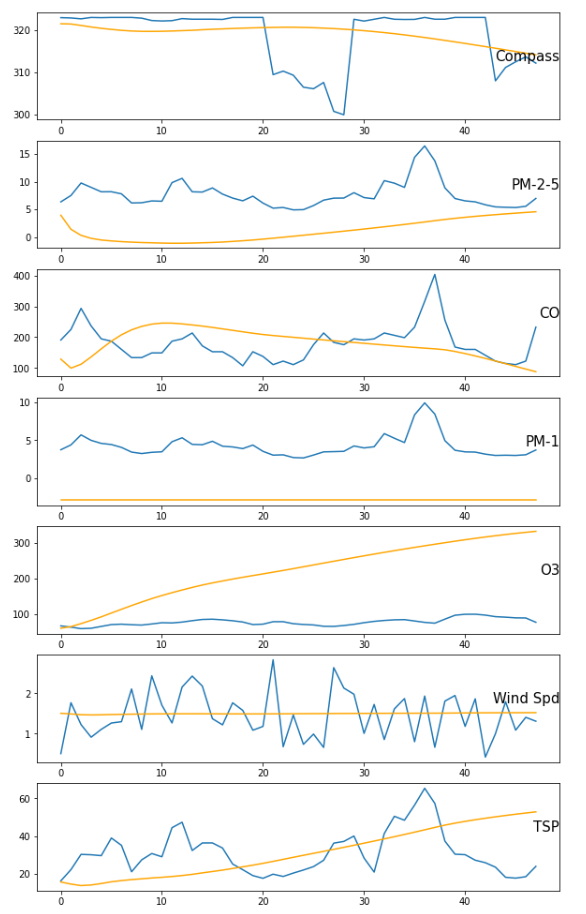
\includegraphics[width=.95\textwidth]{figures/LSTM_test4.png}
    \caption[Compass, PM-2-5, CO, PM-1, O3, Wind Spd và TSP]{Compass, PM-2-5, CO, PM-1, O3, Wind Spd và TSP}
\end{figure}
\newpage
\begin{figure}[H]
    \centering
    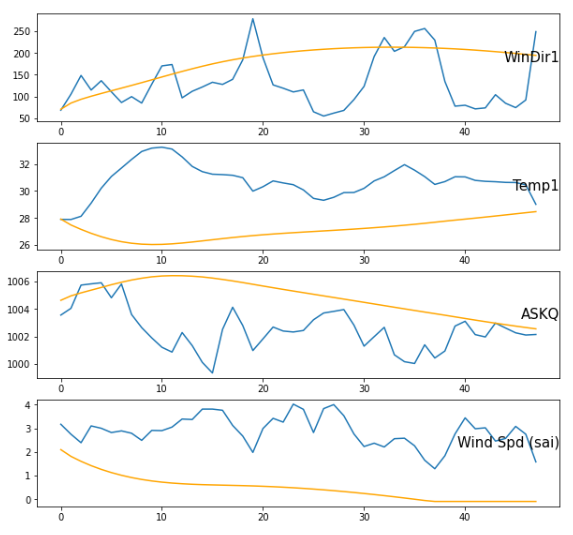
\includegraphics[width=1\textwidth]{figures/LSTM_test5.png}
    \caption[WinDir1, Temp1, ASKQ, Wind-Spd(sai)]{WinDir1, Temp1, ASKQ, Wind-Spd(sai)}
\end{figure}
Nhận xét:
\begin{itemize}
    \item Mô hình LSTM cho MSE và RMSE đều thấp. Sau 200, LOSS giảm dần về 0 và RMSE giảm còn 0.1.
    \item Kết quả dự đoán so với kết quả test không khớp nhau vẫn còn chênh lệch khá nhiều.
    \item Một số cột kết quả dự đoán cho giá trị là một đường thẳng.
    \item Mặc dù cả LOSS và RMSE đều thấp nhưng mô hình dự đoán kết quả lại không tốt.
    \item Mô hình không phù hợp với bộ dữ liệu.
\end{itemize}
\newpage
\subsection{Mô hình VARMAX}
\begin{enumerate}
    \item Đánh giá mô hình:
    \begin{itemize}
    \item Giá trị MSE của mô hình sau khi huấn luyện qua 1000 epoch (maxiter = 1000) là \textbf{1031.6635015800691} 

    \item Kết quả đánh giá theo một số cột:
    \begin{figure}[H]
        \centering
        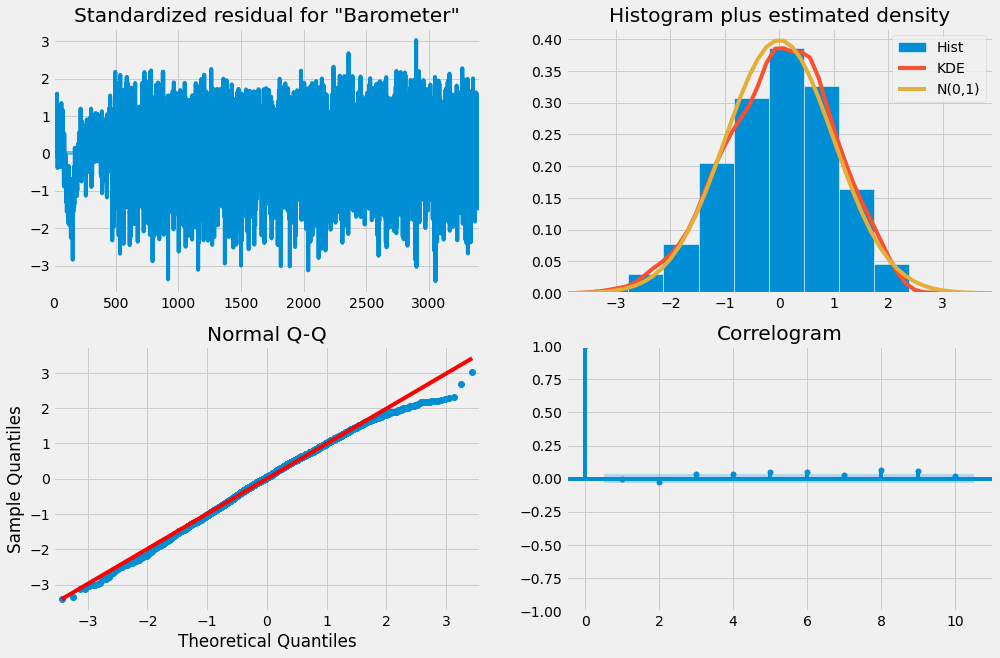
\includegraphics[width=0.75\textwidth]{figures/danhgia1.png}
        \caption[Barometer]{Barometer}
    \end{figure}

    %\begin{figure}[H]
     %   \centering
     %   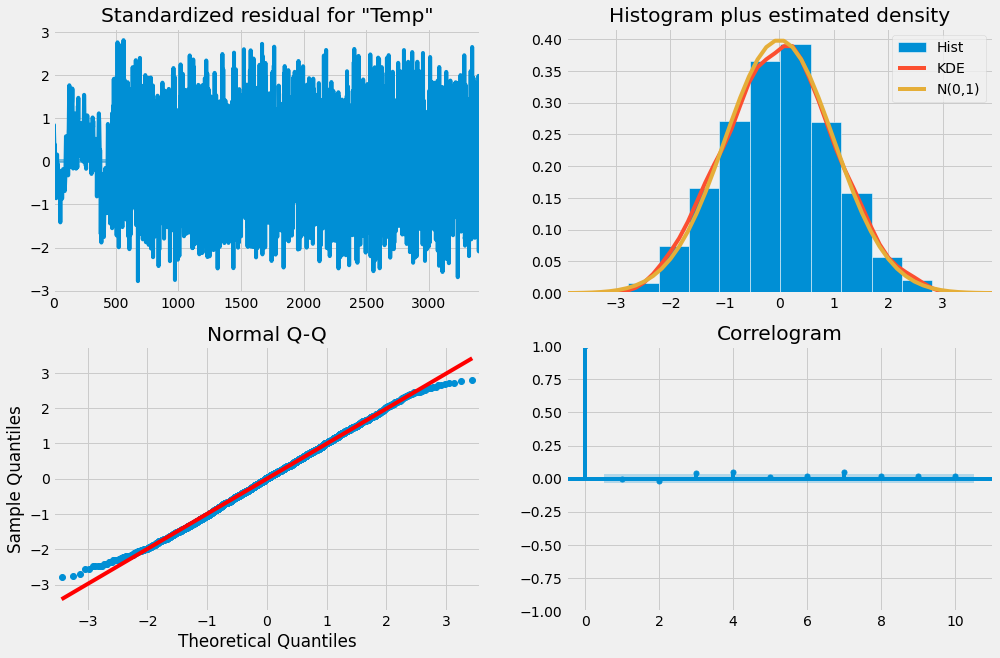
\includegraphics[width=0.7\textwidth]{figures/danhgia.png}
     %   \caption[Temp]{Temp}
    %\end{figure}

    \begin{figure}[H]
        \centering
        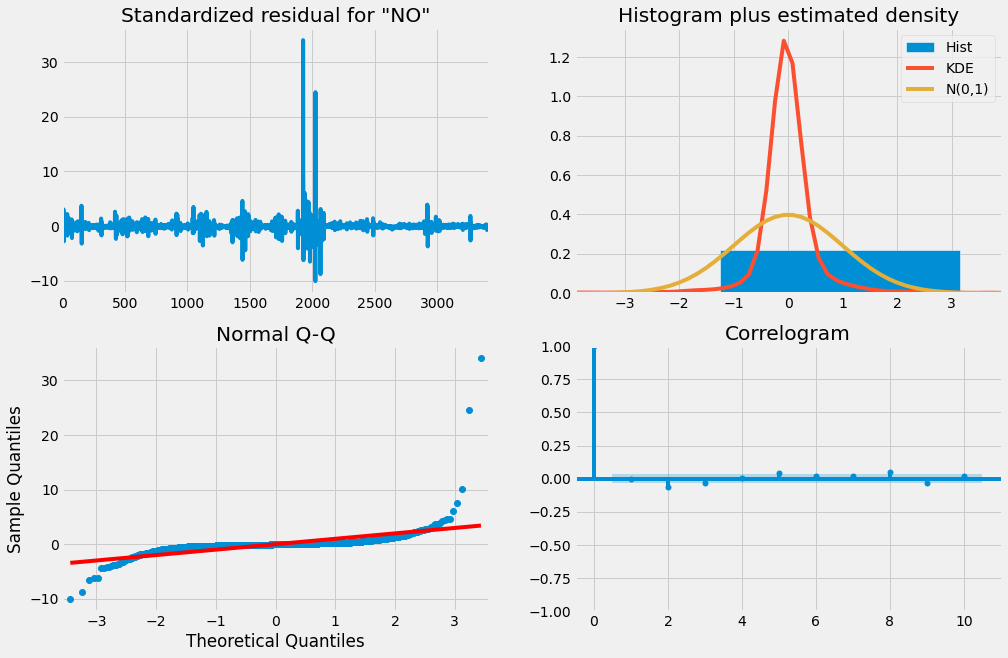
\includegraphics[width=0.75\textwidth]{figures/danhgia3.png}
        \caption[NO]{NO}
    \end{figure}
    
\end{itemize}

    \item Kết quả dự đoán so với tập test
    \begin{figure}[H]
        \centering
        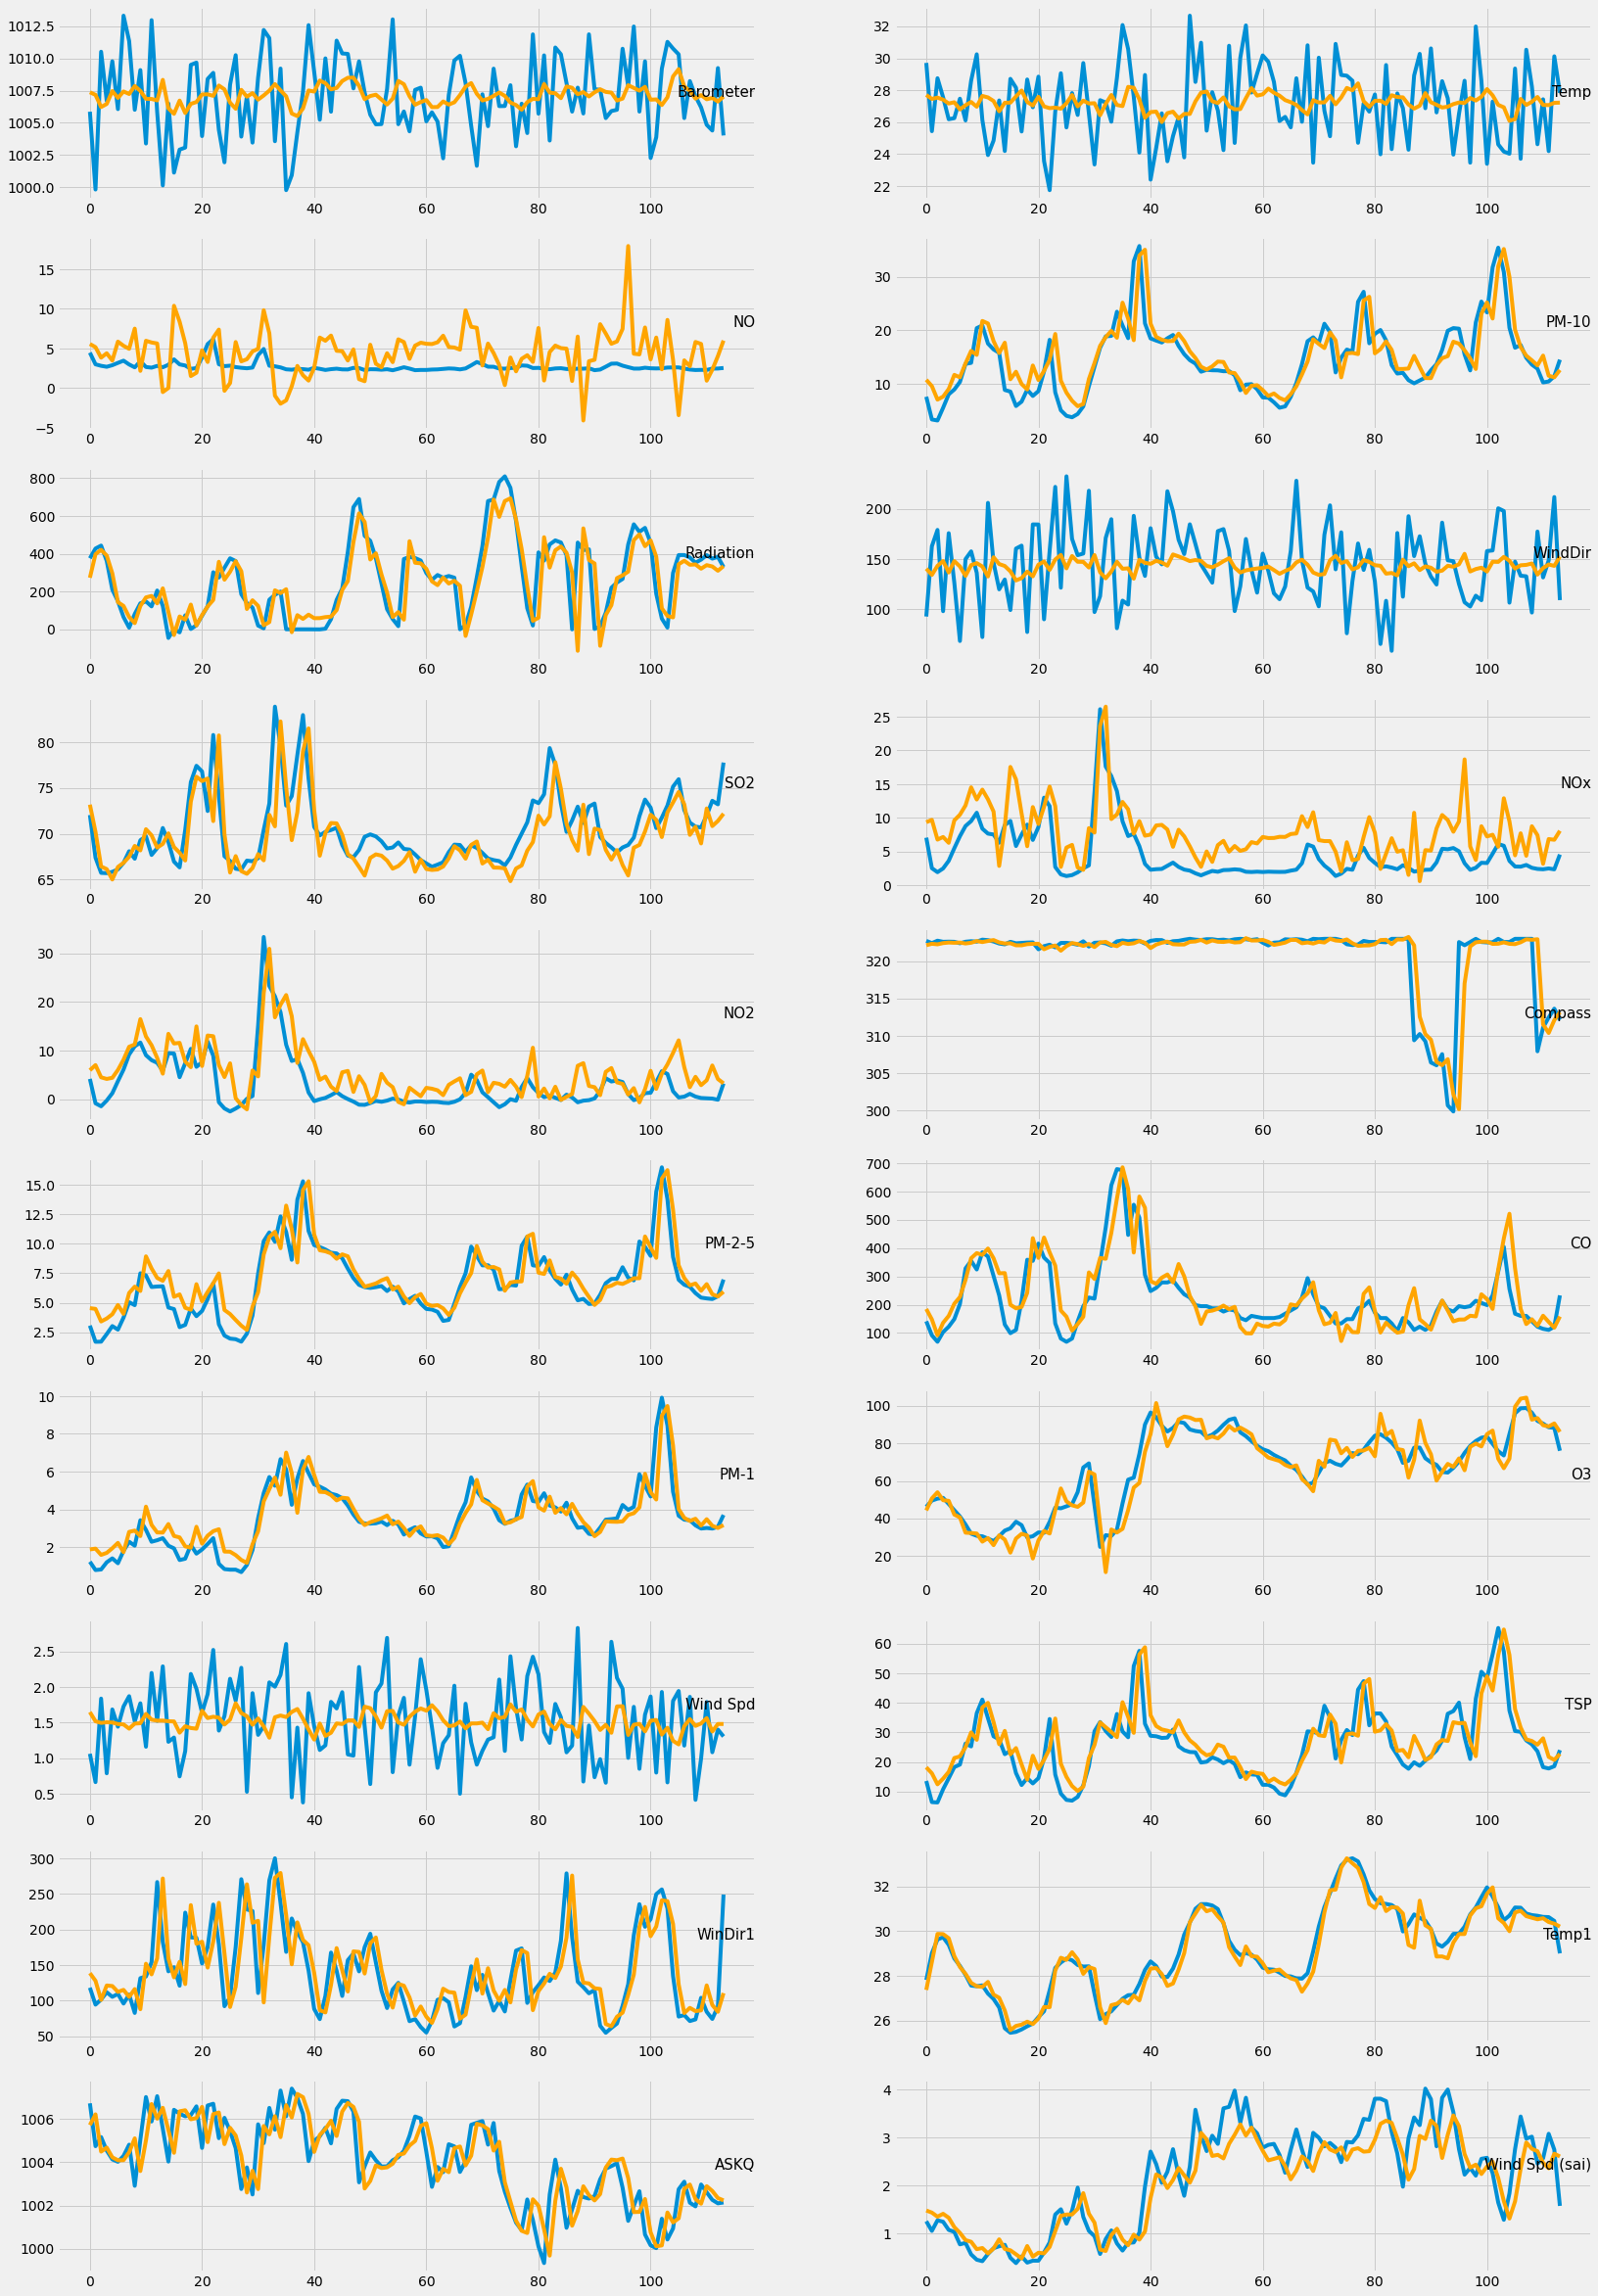
\includegraphics[width=.95\textwidth]{figures/VAR_test.png}
        \caption[Kết quả dự đoán so với tập test]{Kết quả dự đoán so với tập test}
    \end{figure}

    %\item Kết quả dự đoán 48 giờ sau đó
    %\begin{figure}[H]
    %    \centering
    %    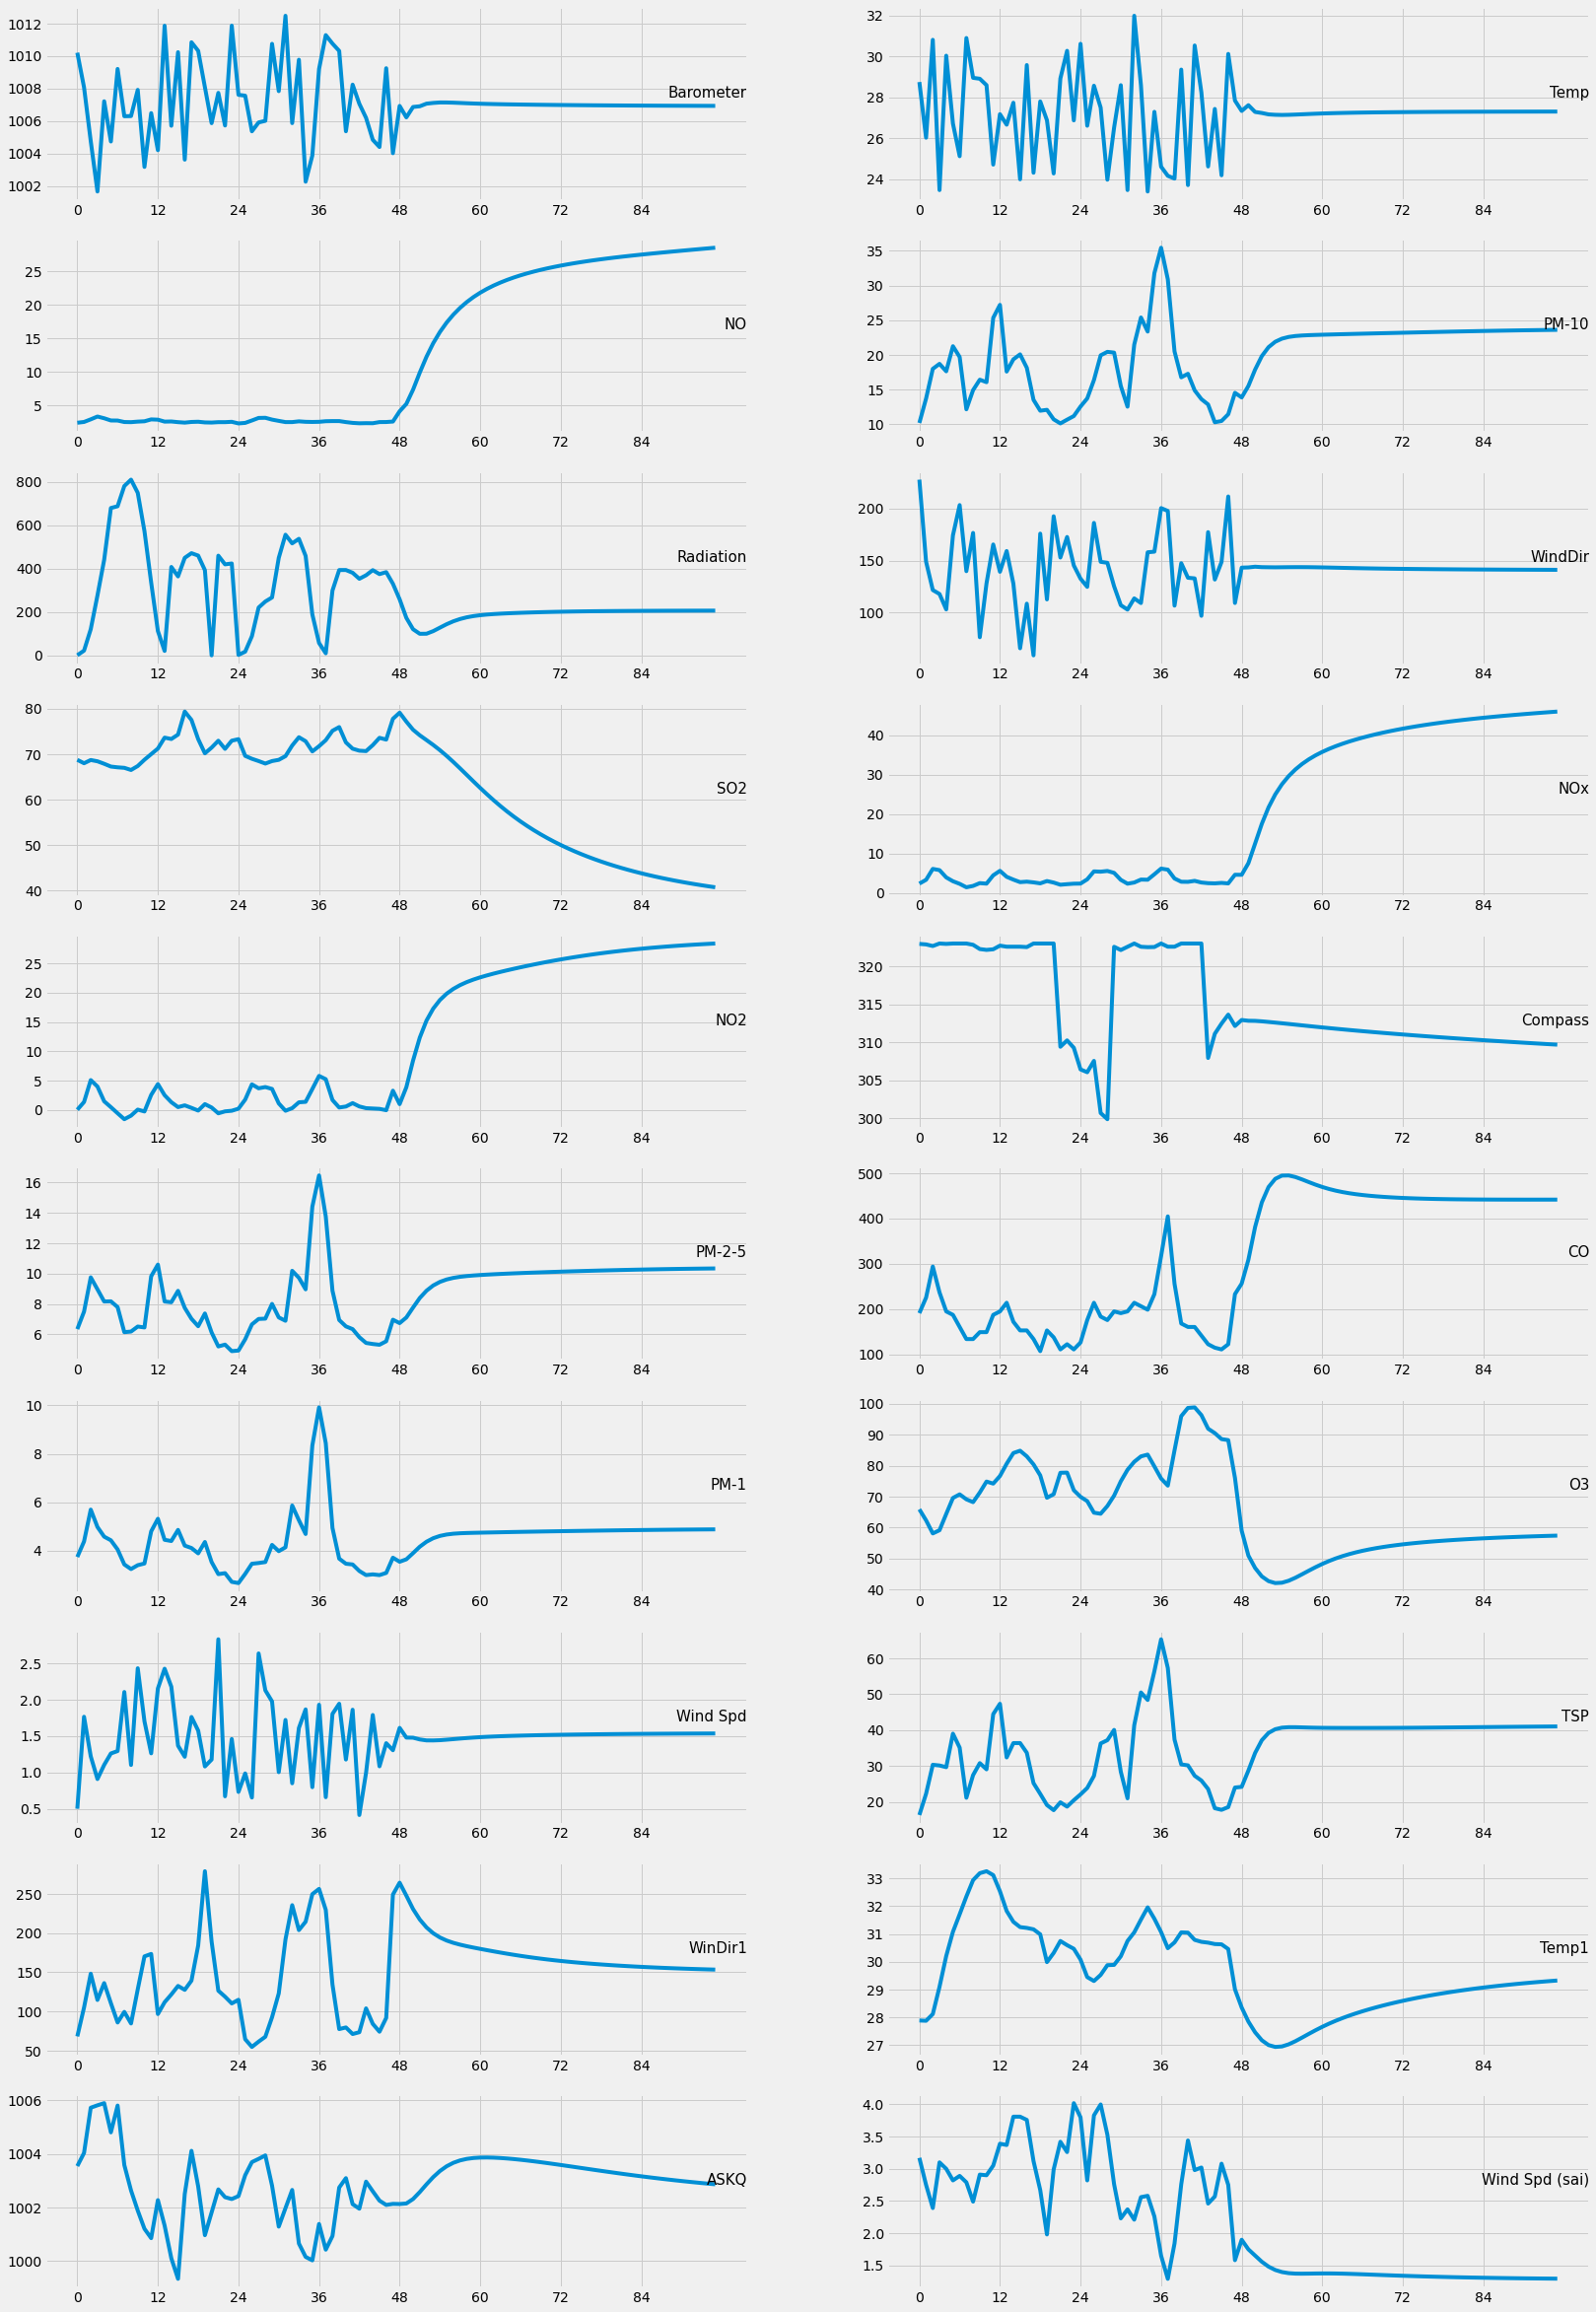
\includegraphics[width=.95\textwidth]{figures/VAR_predic.png}
    %    \caption[Kết quả dự đoán 48 giờ sau đó]{Kết quả dự đoán 48h sau đó}
    %\end{figure}
    %Hình ảnh trên biểu diễn các đồ thị của các cột với dữ liệu 48 giờ cuối của bộ dữ liệu và 48 giờ được dự đoán sau đó.
\end{enumerate}

Nhận xét:
\begin{itemize}
    \item Sau khi huấn luyện qua nhiều lần, thì giá trị MSE của mô hình VARMAX này vẫn khá cao.

    \item Tuy nhiên kết quả dự đoán so với kết quả test khá khớp với nhau trừ một số cột dữ liệu biến động mạnh.

    %\item Đồ thị kết quả dự đoán sau 48 giờ khá ổn định so với 48 giờ trước đó.

    \item Mô hình vẫn cần cải thiện để phù hợp với bộ dữ liệu hơn nữa.
\end{itemize}

\noindent \textbf{Nhận xét chung}: Với các kết quả thu được từ hai mô hình đã thử nghiệm LSTM và VARMAX trên, nhận thấy mô hình VARMAX là phù hợp với bộ dữ liệu hơn.
	\chapter{KẾT LUẬN}
Trong phạm vi nội dung của bài tập lớn, một số nội dung mà nhóm chúng em đã đạt được:
\begin{itemize}
    \item Thành công trong việc giới thiệu mô hình dự đoán chuỗi thời gian LSTM và mô hình VARMAX. 
    \item Ứng dụng được vào bài toán dự đoán chất lượng không khí.
\end{itemize}
Với những kết quả đạt được, bài tập lớn có nhiều tiềm năng ứng dụng trong nhiều bài toán khác nhau về chuỗi thời gian. Một số hướng phát triển tiếp theo của đồ án:
\begin{itemize}
    \item Cải thiện độ chính xác của mô hình và ứng dụng vào nhiều lĩnh vực khác nhau, ví dụ: dự báo giá chứng khoán, dự đoán doanh số bán hàng, v.v...
    \item Phát triển thêm các biến thể của LSTM như Gated Recurrent Unit (GRU), Depth Gated RNNs hay Clockwork RNNs
\end{itemize}


\newpage
\begin{center}
   \textbf{\LARGE{Tài liệu tham khảo}}
\end{center}
\addcontentsline{toc}{section}{Tài liệu tham khảo}
\begin{enumerate}
    \item Joos Korstanje, \textit{Advanced Forecasting with Python}.
    \item B. Brockwell and R. Davis, "Time series: Theory and methods", Springer-Verlag, 1987.
    \item S. Hochreiter and J. Schmidhuber, "Long short-term memory", \textit{Neural computation}, vol. 9, pp. 1735-80, 12 1997.
    \item \url{https://viblo.asia/p/machine-learning-thu-lam-nha-thien-van-du-bao-thoi-tiet-djeZ1xYmKWz}
    
    \item \url{https://www.statsmodels.org/dev/examples/notebooks/generated/statespace_varmax}
    
    \item \url{https://vi.wikipedia.org/wiki/Sai_s%E1%BB%91_to%C3%A0n_ph%C6%B0%C6%A1ng_trung_b%C3%ACnh}
\end{enumerate}



 
    \addcontentsline{toc}{chapter}{TÀI LIỆU THAM KHẢO}
	%\bibliographystyle{plain}
	%\bibliographystyle{ieeetr}
	%\bibliography{References.bib}
	
\end{document}